\documentclass[12pt, a4paper, twoside, openright]{book}

\usepackage{vuwthesis} % sets up some local things, mostly the front page

\usepackage{palatino} % sets palatino as the default font

\usepackage{url} % for typesetting urls

\usepackage{amsmath}

\usepackage[parfill]{parskip}

\usepackage{graphicx}

\usepackage{amssymb}

\usepackage{multirow}

%\renewcommand{\baselinestretch}{1.00}


\begin{document}

\frontmatter
% Book style knows about front matter
% Report style doesn't so you need to set roman numbering etc yourself :-(

%%%%%%%%%%%%%%%%%%%%%%%%%%%%%%%%%%%%%%%%%%%%%%%%%%%%%%%

\title{Dirichlet Methods for Bayesian Source Detection in Radio Astronomy Images}
\author{Anna Friedlander}

\subject{Computer Science}
\abstract{The sheer volume of data to be produced by the next generation of radio telescopes --- exabytes of data on hundreds of millions of objects --- makes automated methods for the detection of astronomical objects (``sources") essential. Of particular importance are low surface brightness objects, which are not well found by current automated methods.

This thesis explores Bayesian methods for source detection that use Dirichlet or multinomial models for pixel intensity distributions in discretised radio astronomy images. A novel image discretisation method that incorporates uncertainty about how the image should be discretised is developed. Latent Dirichlet allocation --- a method originally developed for inferring latent topics in document collections --- is used to estimate source and background distributions in radio astronomy images. A new Dirichlet-multinomial score, indicating how well a region conforms to a well-specified model of background versus a loosely-specified model of foreground, is derived. Finally, latent Dirichlet allocation and the Dirichlet-multinomial score are combined for source detection in astronomical images. 

The methods developed in this thesis perform source detection well in comparison to two widely-used source detection packages and, importantly, find dim sources not well found by other algorithms.
}

\mscthesisonly


%%%%%%%%%%%%%%%%%%%%%%%%%%%%%%%%%%%%%%%%%%%%%%%%%%%%%%%




\maketitle

\chapter*{Acknowledgments}\label{C:ack} 

Marcus, thank you for your generosity with your time and ideas, for believing in me, and always encouraging me to do better.

Thank you Melanie for the privilege of working alongside you and your team of radio astronomers.

Thank you Chris for all your practical assistance and insightful suggestions.

I gratefully acknowledge the financial assistance provided by a KAREN Capability Build Fund grant in support of radio astronomy.

To my husband Karl: thank you for your support, encouragement, and unwavering optimism.

To my son Malachi: your beautiful smile, kind heart and cheeky sense of humour always brighten my day.


\tableofcontents

\listoffigures

\listoftables

%%%%%%%%%%%%%%%%%%%%%%%%%%%%%%%%%%%%%%%%%%%%%%%%%%%%%%%

% book style knows about mainmatter
% if you are using report style you will have to rest page numbering etc.
\mainmatter

%%%%%%%%%%%%%%%%%%%%%%%%%%%%%%%%%%%%%%%%%%%%%%%%%%%%%%%

% individual chapters included here

\chapter{Source detection in radio astronomy}\label{C:intro}
The sheer volume of data to be produced by next generation radio telescopes makes automated methods for the detection of astronomical objects (``sources") essential. Current methods require time-intensive parameter tuning and do not find all sources, particularly scientifically interesting low surface-brightness objects.

This thesis explores Bayesian methods that use Dirichlet or multinomial models for pixel intensity distributions in source detection in discretised radio astronomy images.

The methods developed in this thesis exploit the consistency of image background, while minimising the problems inherent in modelling the diversity of astronomical objects. The posterior probability that a given region is source or background is inferred, avoiding the difficulties in approaches based on comparing ``typical" exemplars of source and background.

\section{Source detection in radio astronomy}
Existing automated approaches to detecting scientifically important astronomical objects require time-intensive manual parameter tuning, and manual post-processing by an astronomer. The sheer volume of data to be produced by the next generation of radio telescopes --- exabytes of data on hundreds of millions of objects --- will make efficient and timely detection of astronomical objects by such manually intensive processing at best impracticable and at worst impossible. Fully automated approaches that do not require manual tuning and post-processing are therefore essential to finding objects of interest in astronomical images \cite{norris2011emu}.

Further, current algorithms for automatic source detection are not fully adequate to find all objects of interest. Spatially extended sources, particularly those that are faint, are poorly handled by existing automated approaches, as are sources in the presence of artefacts, and sources in images in which the signal-to-noise ratio varies across the image \cite{hollitt2012feature, norris2011emu, norris2012radio}.

\subsection{Characteristics of radio astronomy images}

Radio astronomy images can be thought of as primarily background with an unknown number of spatially extended sources. Identifying the sources requires distinguishing them from background, a task made difficult by the diversity of pixel intensities within and between sources. In general, source pixels are brighter than background pixels, though there is considerable overlap between background and source intensity ranges. 

The intensity of background pixels in radio telescope images is non-uniform, but follows a Gaussian distribution in local areas. The variability of background however is lower than that of sources and in that sense it is easier to identify.

The noise in radio astronomy images varies over an image. Images typically display more noise around their edges (for example, see Figure \ref{fig:background-var} in Chapter \ref{C:1D}).

Sources in radio astronomy images can be divided into the following classes:
\begin{itemize}
\item Point sources (Figure \ref{fig:pointsource}), which are unresolved sources in an image; at or below the resolution
element of a telescope. Point sources are abundant in radio astronomy images. They are relatively bright and not spatially extended, and are well-found by existing algorithms\footnote{Hancock \textit{et. al.} \cite{hancock2012compact} report that $\sim 99\%$ of point sources are found by widely used source detection packages (that is, a $\sim 1\%$ false negative rate); similarly $\sim 99\%$ of reported point sources are actual point sources (a $\sim 1\%$ false positive rate).}.
\item Galaxy clusters and associated structures, which are of interest to astronomers. These include:
	\begin{itemize}
	\item Radio galaxies consist of a small, circular, central source from which two, roughly symmetrical, elliptical lobes emanate 180 degrees from each other. The central source is typically brighter than the lobes. Radio galaxies such as the linear source Centaurus A (Figure \ref{fig:centa}) may be bright and extended, or they may be diffuse, extended, low surface brightness sources. One or more of the lobes or central source may be absent or may be distorted. A galaxy's symmetry may be distorted, and lobes may be warped and may differ in size, shape, and brightness. One lobe may appear brighter than the other. Unrelated objects (for example, point sources) may appear on or near the galaxy. Tailed radio galaxies are a sub-class of radio galaxies (Figure [REF]). 
	\item Radio relics (found on the periphery of clusters) appear as dim, diffuse, extended single or double arcs (Figure \ref{fig:radio-relic}).
        \item Radio halos (found around the centres of galaxy clusters) are diffuse, circular structures.
	\end{itemize}
\item Supernova remnants (SNRs; Figure [REF]) are also of interest to astronomers. SNRs generally appear as hollow circular rings, although regions of the rings are often occluded, and symmetry may be distorted. Old and near SNRs appear faint, diffuse and large in images. Young and distant SNRs may be miss-classified as point sources.
\end{itemize}

Artefacts in images appear as bright circles, rings and radial lines. Artefacts will be less prevalent in next generation radio telescope images, due to the increased number of elements in next generation arrays \cite{norris2011emu}. 

A number of characteristics of astronomical objects of interest to astronomers make the object-detection task non-trivial. These include distorted symmetry and other variations in the appearance of sources, occlusions, and low surface-brightness, particularly in diffuse objects with intensities close to noise.

\begin{figure}
\centering
\makebox[\textwidth][c]{\includegraphics[width=1.0\textwidth]{IMAGES/pointsource.png}}
\caption[Point source]{\textbf{A point source}. The red contours show the $1.4$ GHz radio data and the blue show the $2.4$ GHz data overlaid on the optical image from the Digitized Sky Survey. The resolution of these radio data are $8.8 \times 4.6$ arcseconds at position angle of $2.4$ degrees and $5.0 \times 2.6$ arcseconds at $2.5$ degrees at $1.4$ and $2.4$ GHz, respectively. Despite that the optical host galaxy is clearly seen the radio data are unresolved at both frequencies and so this is a point source in a radio image \cite{johnston2008radio}.}
\label{fig:pointsource}
\end{figure}

\begin{figure}
\centering
\makebox[\textwidth][c]{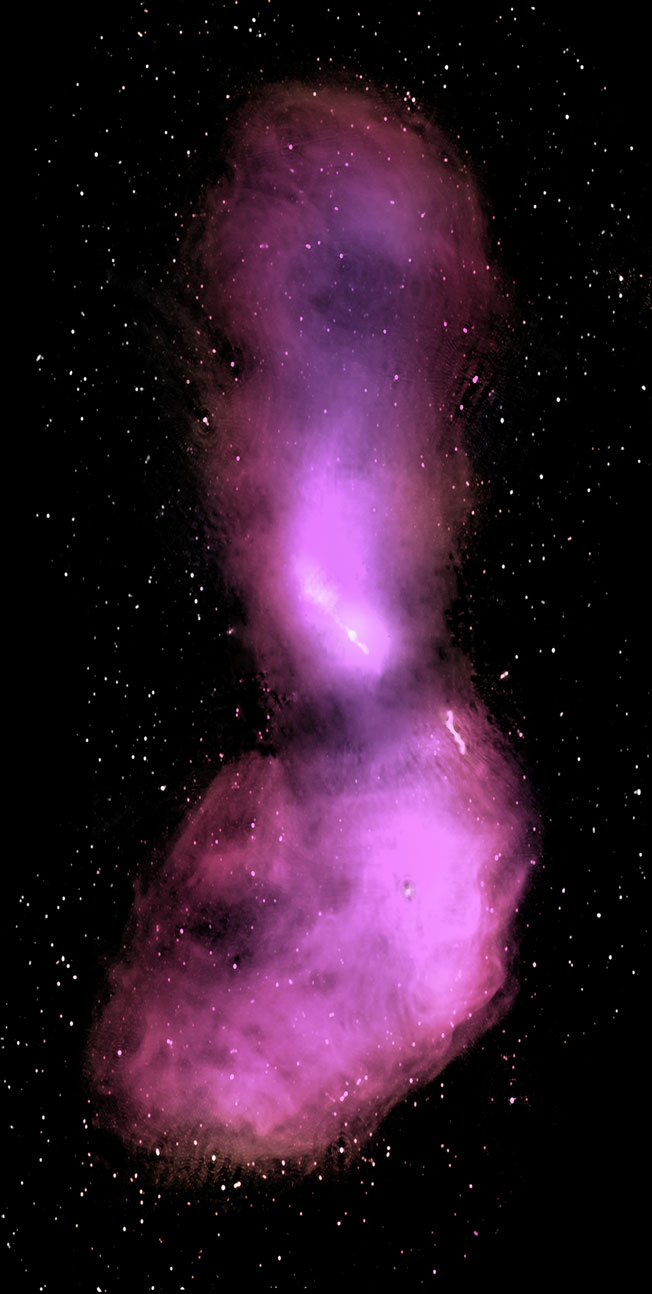
\includegraphics[width=0.7\textwidth]{IMAGES/casa2_lg.jpg}}
\caption[Radio galaxy]{\textbf{A radio galaxy}. Centaurus A is the nearest powerful radio galaxy of the Fanaroff-Reilly class 1 radio galaxies, which typically have jets at 180 degrees \cite{feain2011radio}. }
\label{fig:centa}
\end{figure}


%[Tailed radio galaxy] The tailed radio galaxy PKS J0334-3900

\begin{figure}
\centering
\makebox[\textwidth][c]{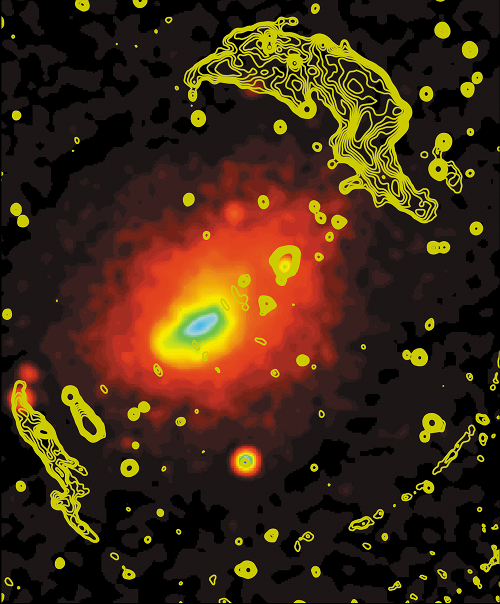
\includegraphics[width=1.0\textwidth]{IMAGES/radio-relics.jpg}}
\caption[Radio relic]{\textbf{A radio relic}, shown by yellow contours \cite{johnston2003detection}.}
\label{fig:radio-relic}
\end{figure}

%SNR figure \cite{zanardo2013high}


\subsubsection{Image format}

Radio telescope images are typically stored in FITS (Flexible Image Transportation System) format. For the astronomical images used in this thesis, image data is stored in two dimensional arrays of pixel intensities with implicit Cartesian coordinates. Pixel intensity values are continuous, and range from small positive to small negative values in any given image. Image meta-data including information about the equatorial coordinates of the image is also stored with this format \cite{wells1981fits}. 

\subsection{Existing approaches to source detection}

An ideal source-finding algorithm should locate regions in an image that differ from the background and are unlikely to have arisen by statistical variation in noise. False positives are more acceptable than than false negatives (as astronomers can do post-processing to confirm and characterise sources), however, a large number of false positives would make output difficult to interpret at best and unusable at worst.

In a 2012 review, Masias \emph{et. al.} \cite{masias2012review} characterised current approaches to automated and semi-automated source detection in astronomy as a two-step process: an image transformation step followed by a detection step. 

Masias \emph{et. al.} divided approaches in the transformation step into basic transformation methods, Bayesian approaches, matched filtering, and multi-scale approaches. Basic transformation methods predominate, and include median filtering, local thresholding using information such as pixel intensity mean and standard deviation, Gaussian image convolution, dilation and erosion, and template matching.

Bayesian approaches transform pixel intensity data to a probability map indicating regions where sources are likely to be located (for example: \cite{feroz2008multimodal}; also see Section \ref{sec:Bayesian-src-det} below). Matched filtering involves convolving an image using an expected source profile as a filter (for example: \cite{torrent2010detecting}), while multi-scale approaches work by applying a transform to decompose images into different frequencies (for example: \cite{peracaula2011segmentation}). 

In the detection step Masias \emph{et. al.} categorised the majority of methods into thresholding (local or adaptive) and local peak search (region growing from peaks in, for example, pixel intensities). The authors also list a small number of ``other" techniques (neural networks, watershed transform, contrast radial function, and connected component trees).

The majority of automated source detection algorithms can therefore be described as flood-filling or region-growing driven by (possibly transformed) pixel intensities \cite{masias2012review}.

Such intensity based thresholding algorithms often require a parameter to be set (either manually or automatically as part of the algorithm) that restricts the sources to be found as those that are at least as bright as some threshold: typically $3 \sigma$ or $5 \sigma$ above root mean square (rms) noise. However, as noted earlier in this chapter, some of the most scientifically important objects in astronomy are dim, low surface brightness sources, with intensities in the range of background noise \cite{norris2011emu}. Restricting the search for sources that contain pixels above a particular threshold restricts the set of sources that may be found. This is due to the nature of thresholding algorithms: if the search is not restricted in this way, far too many background regions will be identified as ``sources", and the output will be unusable.

Threshold-based algorithms are often reported to have very high rates of true detections with very low rates of false detections and missed sources. However, these rates must be taken with caution, as they are often restricted to the sub-set of sources in an image above a particular brightness. For example, Hancock \textit{et. al.} \cite{hancock2012compact} report perfect detection rates with no false detections or missed sources --- in the case of simulated point sources $10 \sigma$ above rms noise. 

The source detection algorithms developed in this thesis are evaluated against two source detection software packages commonly used in radio astronomy: Duchamp \cite{whiting2012duchamp} and BLOBCAT \cite{hales2012blobcat}; both of which perform pixel-intensity based thresholding in the transformation step and flood-filling in the detection step.

\subsection{Bayesian source detection methods}\label{sec:Bayesian-src-det}

Beside the many thresholding and flood-filling / region-growing algorithms, there are a small number of Bayesian source detection algorithms \cite{masias2012review}.

Most of these Bayesian source detection algorithms use Markov-chain Monte Carlo sampling (MCMC) to estimate the relative probability that each pixel (or pixel grouping) in an image is a background pixel or a source pixel \cite{feroz2008multimodal, masias2012review}. 

Savage and Oliver \cite{savage2007bayesian} used MCMC for source detection in infrared astronomical images. Each pixel was labelled with the relative probability of being a background pixel or a source pixel, with a flat and uniform background model, and a source model consisting of background plus a circularly symmetric Gaussian point source of known size. This labelling yields a probability map which can be used to find local maxima (subject to some threshold) corresponding to locations of point sources. Once the location of putative sources is found by this method, the nature of the source is identified: MCMC sampling is used to find the best-fit model of uniform background, point source, or extended source models (where point sources are circularly symmetric and of known size, and extended sources are circularly symmetric with variable size).  

Similarly, Hobson and McLachlan \cite{hobson2003bayesian} performed Bayesian model selection using MCMC to explore the parameters of background and source models, with a source model of circularly symmetric Gaussian-shaped objects and a background model of Gaussian noise. They present two versions of the algorithm: one in which all sources are found simultaneously, and one in which sources are found iteratively. A significant speed up to this technique is presented in Carvalho \textit{et. al.} \cite {carvalho2009fast}, in which multiple local maximisation of the posterior distribution replaces sampling, and a Gaussian approximation to the posterior is used for the evaluation of Bayesian evidence in model selection.

Guglielmetti \textit{et. al.} \cite{guglielmetti2009background} developed a Bayesian source detection method for X-ray data. They used a two component mixture model where an astronomical image is assumed to consist of a smooth background with additive source signal; therefore the two models are $1.$ background plus noise and $2.$ background plus source plus noise.

Feroz and Hobson \cite{feroz2008multimodal} developed one of the few non-MCMC based Bayesian source detection algorithms. They used the Bayesian model selection algorithm nested sampling \cite{skilling2004nested}, which they argue outperforms MCMC based methods, and is computationally less expensive. Similarly to other Bayesian source detection methods, circularly symmetric Gaussian-shaped sources are assumed.

The Bayesian source detection methods developed in this thesis have some similarities with the existing algorithms in astronomy. For example, in Chapter \ref{C:LDA}, in latent Dirichlet allocation (LDA), Gibbs sampling is performed on individual pixels which are probabilistically assigned background or source labels, with flood-filling performed on the transformed image to identify islands of source pixels. In Chapters \ref{C:1D} and \ref{C:2D}, a Bayesian score (``DM-Score") is derived to iteratively find Gaussian elliptical shaped regions that conform to a source model (or differ from a background model).

In contrast to the existing Bayesian source detection methods however, source and background are modelled as distributions over ranges of pixel intensities. As with the existing Bayesian algorithms, the DM-Score assumes a parametrised form for astronomical sources and estimates these parameters from a posterior distribution, however sources are not assumed to be circularly symmetric or of a particular size. Under LDA, no particular size or shape of sources is assumed.

It is worth noting that in several cases, these Bayesian source detection methods are tested on simulated data in which the sources are generated with the same parameters as the model of source used in the detection methods. For example \cite{feroz2008multimodal,hobson2003bayesian,savage2007bayesian} generate circularly symmetric Gaussian sources of a particular size, and use a circularly symmetric Gaussian of that size as a source model. Using the same parameters for simulated source and the method's source model is likely to artificially inflate the success of the model, and is unjustified in the case of radio astronomy data, where sources can take a great variety of shapes and sizes.

\section{Outline of the thesis}

Within the framework provided by Masias \emph{et. al.} \cite{masias2012review}, the source detection algorithms in this thesis can be characterised as follows:
\begin{itemize}
\item \textbf{Image transformation step}: the continuous valued pixel intensities in astronomical images are converted to discrete values by histogram binning or discretisation. This process is described in \textbf{Chapter \ref{C:BIN}}.
\item \textbf{Detection step}: two approaches are taken:
    \begin{itemize}
    \item Background and source models are inferred using the topic modelling technique latent Dirichlet allocation, these models are used to classify pixels according to which model they were most likely generated by. Flood-filling is then performed to find contiguous regions of ``likely to be source" pixels. The use of LDA for source detection is described in \textbf{Chapter \ref{C:LDA}}. Results of this technique as compared to results obtained by a standard source-detection package are presented.
    \item A Dirichlet-multinomial ``score" (DM-Score) is derived, and, given a background model and a loosely specified source model, gradient ascent is performed to find peaks in the score indicating regions that are unlikely to be background. The derivation of the DM-Score is outlined in \textbf{Chapter \ref{C:1D}}. Results of the DM-Score on real and simulated data are presented in  \textbf{Chapter \ref{C:2D}}.
\end{itemize} 
\end{itemize} 

A combined LDA DM-score technique is described and evaluated in \textbf{Chapter \ref{C:2D-LDA}}. The work in the thesis and its limitations are summarised and possible future work suggested in \textbf{Chapter \ref{C:con}}.

\section{Original contributions}

The contributions of this thesis are as follows:
\begin{itemize}
\item A novel method for incorporating uncertainty about where bin borders should be located in discretised data is introduced in \textbf{Chapter \ref{C:BIN}}.
\item The first use of the topic modelling technique latent Dirichlet allocation (developed to extract latent topics from collections of documents) in source detection in astronomical images is described in \textbf{Chapter \ref{C:LDA}}. This application of LDA to source detection differs from that taken in previous approaches to the segmentation of non-astronomical images in that it relies only on pixel intensity and location, whereas previous approaches employ techniques to extract image interest points and pre-segment images before applying LDA.
\item A new Dirichlet-multinomial score, indicating how well a region conforms to a model of background versus a model of foreground is derived in \textbf{Chapter \ref{C:1D}}.
\item LDA output is utilised in the DM-Score in \textbf{Chapter \ref{C:2D-LDA}}.
\end{itemize}

\chapter{Discretising images}\label{C:BIN}

Astronomical images have continuous-valued pixel intensities. These continuous values can be converted to discrete values --- ``discretised" --- by histogram binning. 

Histogram binning is a method of mapping a large number of continuous values (in this case, pixel intensities) to a smaller set of discrete values (or ``bins"), where all values within a range are assigned a discrete label representing that range \cite{yang2010discretization}.

Discretisation of continuous pixel intensity values makes it possible to model the data according to a multinomial distribution, and to use the Dirichlet distribution, which is the conjugate prior for the multinomial distribution \cite{diaconis1979conjugate,frigyik2010introduction,johnson1997discrete,kotz2004continuous}. This allows the use of the topic modelling technique latent Dirichlet allocation \cite{blei2003latent} (LDA; Chapter \ref{C:LDA}) and the derivation of a Dirichlet-multinomial Score (DM-Score; Chapters \ref{C:1D} and \ref{C:2D}). LDA and the DM-Score are combined in Chapter \ref{C:2D-LDA}\footnote{Note that a compound Dirichlet-multinomial distribution is used in both LDA and the DM-Score. In both cases the multinomial parameter is integrated out, leaving only the data and the Dirichlet hyperparameter. LDA estimates a conditional distribution while the DM-Score calculates a marginal joint distribution \cite{blei2003latent, ng2011dirichlet}.}. 

Discretisation is a simplification and reduction in the complexity of the information in the data. It is therefore important that the process of discretisation does not destroy information essential to the task at hand. In the case of source finding in radio astronomy images, it is important that information that can be used to discriminate source pixels from background pixels is not lost. Though discriminative ability may be decreased by discretisation, an ideal discretisation retains or improves discriminative accuracy \cite{kotsiantis2006discretization,liu2002discretization}.

In this chapter, simple data partitioning methods for defining histogram bins for discretisation are described in Section \ref{sec:binning-strategies}. A novel way of ``softening" bin borders to incorporate uncertainty about the location of partition-points in the data is described in Section \ref{sec:dirichlet-borders}. An exploratory approach to source finding in discretised images is described in Section \ref{sec:multi}.

\section{Histogram binning strategies}\label{sec:binning-strategies}
Histogram binning is the simplest of a range of discretisation methods \cite{kotsiantis2006discretization,liu2002discretization,yang2010discretization}.

The majority of existing discretisation methods are supervised (using a training set of instances with known class labels) \cite{kotsiantis2006discretization,liu2002discretization,yang2010discretization}; these methods are not appropriate for radio astronomy images as the class (source or background) of an image's pixels is not known \textit{a priori}. 

Of the few unsupervised algorithms, cluster-based \cite{chmielewski1996global} and dynamic-qualitative \cite{lopez2000dynamic} --- both of which seek to reduce within-interval variation and maximise between-interval variation --- would be appropriate, but, given the time-consuming nature of these algorithms (particularly relative to histogram binning), neither is practical \cite{yang2010discretization}.

A histogram of pixel intensities can be constructed by assigning each pixel in an image to an interval or ``bin" on the basis of its intensity, where bins are ranges of intensity values defined\footnote{Note that some authors use the definition $(min_k, max_k]$, i.e., $x \in k$ if $min_k < x \le max_k$ \cite{kotsiantis2006discretization}.} as $[min_k, max_k)$. A pixel $x$ falls into bin $k$ if $min_k \le x < max_k$ (except in the case of the last/top bin $K$, which is defined as $[min_K, max_K]$: a pixel $x$ is assigned bin $K$ if $min_K \le x \le max_K$). For adjacent ranges $[min_i, max_i)$ and $[min_j, max_j)$, $max_i \le min_j$ and so each data instance falls into exactly one bin; coverage is ensured by setting $min_j = max_i$.

In order to discretise intensity values by histogram binning, bin borders (values that define $min_k$ and $max_k$ for each bin $k \in K$) must be defined. The number of bins must also be set (either manually, or by the binning method itself). 

A simple way to create bins in data is to partition the data on the basis of either interval-width or bin-occupancy. These methods are described below.

\subsection{Width-based partitions}\label{sec:width}
Width-based methods divide the number-line between $x_{min}$ and $x_{max}$  where $x_{min}$ is the minimum pixel intensity value in the data, and $x_{max}$ is the maximum value \cite{yang2010discretization}.

\subsubsection{Equal width partitions}\label{sec:wid}
One of the simplest ways to partition data into $K$ bins is to create $K$ equal width partitions in the data range $[x_{min},x_{max}]$. The width of intervals is defined as $w = (x_{max} - x_{min})/K$, and the bin are defined at $[x_{min}, x_{min}+w), [x_{min}+w, x_{min}+2w), .. ,[x_{min}+(K-1)w,x_{max}]$. This is an equal partitioning of the number-line between $x_{min}$ and $x_{max}$ \cite{yang2010discretization}.

Equal width discretisation of non-uniformly distributed data may result in an inaccurate representation of the data; for example, outliers may skew the histogram binning \cite{dougherty1995supervised,kotsiantis2006discretization,liu2002discretization}. 

In the case of radio astronomy data, the vast majority of an image's pixels are typically within a small range at the bottom of end of the data range, with a few, relatively small, peaks at the top of the range (see Figure \ref{fig:histo}). This means that an equal width binning scheme will produce many empty bins (which means wasted representation power) and, more importantly, a lack of resolution at the low end of the intensity range. Because many scientifically interesting objects have pixel intensities close to background intensities, equal width binning strategies risk losing information that differentiates background from source pixels. In the case of radio astronomy data, some of these effects may be alleviated with an iterative binning process that removes bright source pixels (outliers) from the histogram binning process once the sources containing these pixels have been identified (for an example, see Chapter \ref{C:2D}).

\begin{figure}
\centering
\includegraphics[width=1.0\textwidth]{IMAGES/histo.png}
\caption[A histogram of pixel intensities in an astronomical image]{\textbf{A histogram of pixel intensities in an astronomical image.} Pixel intensities from the Australia Telescope Large Area Survey Chandra Deep Field-South (ATLAS CDFS) \cite{norris2006deep}, with the \textbf{log} count in each of $1000$ equal width bins. Note the large peak in the low intensities and the outliers in the high intensities.}
\label{fig:histo}
\end{figure}

\subsubsection{Exponentially increasing width partitions}
This problem of including source pixels and background pixels in the same bin(s) may be addressed by exponentially increasing the interval-widths in a partition. 

In this method, intervals are defined recursively with interval $k$ having width $0 < \gamma < 1$ times less wide than interval $k+1$. The last (top) interval $\text{wid}_k$ is defined as $\gamma(x_{max}-x_{min})$, with bin $K-1$ having width $\gamma \text{wid}_k$. For this partitioning method, the number of bins $K$ will be defined by the parameter $\gamma$ and the range of the data.

Depending on the $\gamma$ value used, there may still not be sufficient resolution in the low values to differentiate source from background in radio astronomy images.

\subsection{Frequency-based partitions}\label{sec:occ}
Alternatively, bins may be defined according to their occupancy. In contrast to width-based methods that partition the number line, frequency-based partitions rank the data and make partitions on this ranking \cite{yang2010discretization}.

\subsubsection{Equal occupancy partitions}
Equal occupancy partitions are constructed by dividing the count of pixels $N$ by $K$ bins, to determine the number of pixels $n$ that should fall into each bin $k$. Pixels are allocated to bins by ranking pixels by intensity and partitioning this ranking into $K$ partitions of (approximately, depending on whether $N$ is divisible by $K$) $n$ data points each. The minimum and maximum values in the partition defining the bin boundaries $[min_k, max_k)$ are those of the first and last ranked data points within the partition.

In contrast to width-based partitions, there are no empty bins in equal occupancy partitions (no ``wasted" bins). With respect to astronomical data, low intensity source pixels are less likely to be subsumed into a bin with mostly background pixels (though this is not guaranteed). However, information with respect to the number line, such as bright ``peaks" in the data, is lost, as the resulting distribution of data into bins is not representative of the distribution of the original, non-uniform, data \cite{clarke2000entropy}.

\subsubsection{Exponentially decreasing occupancies}
An exponentially decreasing partitioning of data with respect to occupancy divides the pixel ranking such that each bin $k$ has $0 < \gamma < 1$ times as many pixels as bin $k-1$. 

The first (bottom) bin occupancy $\text{occ}_1$ is created by assigning it the first $\gamma N$-many pixels (where $N$ is the total number of pixels in the data) and defining the minimum and maximum values for bin 1 as the intensities of the first ranked and last ranked pixels within $[min_1, max_1)$ respectively. The rest of the bins are defined recursively (bin $2$ has the next $\gamma \text{occ}_1$-many pixels in the ranking, and so on).

\section{A novel method for softening bin borders}\label{sec:dirichlet-borders}

There are three major problems with the simple discretisation/binning methods described in Section \ref{sec:binning-strategies} for radio astronomy data:
\begin{enumerate}
\item there is a lack of any informed basis for deciding on what bin boundaries to use and so any particular choice amounts to an unjustified assertion; 
\item because radio astronomy data is non-uniform, relevant groupings of values may be split across bins or combined in bins in a way that reduces discriminative power \cite{clarke2000entropy}; and
\item discretisation results in sudden changes at partition values, which introduces variation into the system that did not previously exist --- moreover, data-points that lie near a boundary of a bin are less well represented by that bin than data-points that lie towards the middle of the bin's interval \cite{yang2002non}.
\end{enumerate}

For the source-detection algorithms used in this thesis, bin identities are used to convert pixels in an image or a region in that image into counts in bins. Given that there is a lack of any informed basis for the choice of bin boundaries used, and the problems inherent in binning non-uniform data, it would be more principled to assign proportions of each pixel across a range of bins to reflect uncertainty about which bin a pixel belongs to.

Instead of making a ``hard" assignment of pixels to bins where each pixel is allocated to one bin only, it is possible to create several sets of bins $b \in B$, each of size $K$, with bin sets $b_i$ and $b_j$ having differing partition points. Each pixel would then have a number of ``possible" bin assignments across sets of bins (each pixel $x$ will fall into one bin $k$ for each set of bins $b$).

Given a number of plausible sets of bins $B$, it is possible to count how often a given pixel $x$ appears in each bin $k \in B$. Once normalised (by dividing the counts in each bin by the number of $b \in B$, so that the sum of counts for each pixel $x$ across bins is equal to $1$) this gives a {\it distribution} over all the bins for $x$, which reflects uncertainty about where the borders should lie. 

This solves the problem of the sudden changes at bin borders, and is a method for converting continuous values into distributions over discrete values (counts) in a way that is smooth. It reduces the impact both of the uninformed choice of bins and of any within-class splitting over bins and between-class combining in bins \cite{clarke2000entropy}\footnote{Note that there are existing techniques for transforming continuous attributes to distributions over intervals/bins. Ishibuchi \textit{et. al.} \cite{ishibuchi2004fuzzy} use labelled data and fuzzy logic to create linguistic association rules; Yang and Webb \cite{yang2002non} create overlapping, rather than disjoint, intervals constructed such that a given data-point falls near the middle of its interval, away from interval boundaries. In contrast, the approach developed in this chapter directly addresses uncertainty about where those boundaries lie.}.

\subsection{Creating sets of bins with the Dirichlet distribution}

The Dirichlet distribution is a natural way to create such sets of bins. In this section, the Dirichlet distribution is described, followed by an explanation of how it may be used to create sets of bins.

\subsubsection{The Dirichlet distribution}

Informally, a Dirichlet distribution can be thought of as a distribution over categorical or multinomial probability mass functions (pmfs) of size $K$; or, in other words, a distribution over the ($K-1$) dimensional probability simplex \cite{frigyik2010introduction,ng2011dirichlet}.

Firgyik \textit{et. al.} \cite{frigyik2010introduction} illustrate the intuition behind the Dirichlet distribution using dice. A die can be thought of as a pmf with $K=6$. A given die may be fair (with equal probability of rolling each number) or it may have imperfections that result in a biased or weighted die. A Dirichlet distribution can be thought of as a bag of dice, from which dice may be drawn. The bag may contain dice that are all reasonably fair, biased in some particular manner, or some mixture.

A Dirichlet distribution has a parameter $\boldsymbol{\alpha} = \alpha_1,...,\alpha_K$ and probability density function on the ($K-1$) dimensional simplex:
\begin{align}
f(x_1, ..., x_{K-1};\alpha_1,...,a_K)=\frac{\Gamma(\sum_{i=1}^K \alpha_i)}{\prod_{i=1}^K \Gamma(\alpha_i)}\prod_{i=1}^K x_i^{a_i-1} \label{eq:dir-pdf}
\end{align}
where $\Gamma(.)$ denotes the gamma function; and with $x_i \in [0,1]$, $\sum_{i=1}^{K-1} x_i < 1$, and $x_K = 1 - x_1 - ... - x_{K-1}$ (this parametrisation of the Dirichlet probability density function is due to the fact that the probability density is positive only on the ($K-1$) dimensional simplex and zero elsewhere; the simplex exists in $K$ dimensional space) \cite{frigyik2010introduction,hoadley1969compound,johnson1997discrete,kotz2004continuous,mosimann1962compound,ng2011dirichlet}.

The $\boldsymbol{\alpha}$ parameter controls where the density on the probability simplex lies. In the special case when $\alpha_i = \alpha_j = 1 \; \forall i,j \in K$, the density is uniformly distributed over the simplex. Every multinomial distribution over $K$ is equally likely to be drawn from the Dirichlet distribution with this $\boldsymbol{\alpha}$ parameter. The Dirichlet with uniform $\boldsymbol{\alpha}$ parameter $\alpha_i = \alpha_j < 1$ pushes the density to the corners of the simplex; multinomial distributions with one $x_k$ much greater than all the others (with $(1 - x_k) << 1$ and $x_i << 1 \; \forall i \ne k$) are drawn from the Dirichlet with this $\boldsymbol{\alpha}$ parameter. When $\alpha_i = \alpha_j > 1$, the density lies towards the middle of the simplex. Distributions drawn from the Dirichlet with $\alpha_i = \alpha_j >> 1$ approximate uniform distributions over $K$. When  $\boldsymbol{\alpha}$ parameters are not uniform, the density on the simplex is not symmetric. For non-uniform  $\boldsymbol{\alpha}$ parameters with values $>1$, if  $\alpha_i > \alpha_j$, distributions are likely to be drawn with $x_i > x_j$ \cite{frigyik2010introduction}. Figure \ref{fig:simplex} illustrates these cases.

\begin{figure}
\centering
\includegraphics[width=1.0\textwidth]{IMAGES/simplex.png}
\caption[Dirichlet samples on the simplex]{\textbf{Dirichlet samples on the simplex.} $\boldsymbol{\alpha}$-vectors: $[1,1,1]$ (top left), $[10,10,10]$ (top right), $[0.1,0.1,0.1]$ (bottom left), $[2,5,20]$ (bottom right).}
\label{fig:simplex}
\end{figure}

\subsubsection{Interpreting Dirichlet samples as bin borders}

A single sample from a Dirichlet distribution with an $\boldsymbol{\alpha}$-vector of $K$ components yields a $K$-element vector $\mathbf{x}$ for which $\sum_{k=1}^K x_k = 1$ and all $x_k > 0$ (such as $\mathbf{x}=[0.1,0.7,0.2]$ with $K=3$). The cumulative sum of the elements of $\mathbf{x}$, denote $\mathbf{x}_d$, can be interpreted as partition-points over $[0,1]$ (such as $\mathbf{x}_d = [0.1,0.8,1.0]$). 

To translate $\mathbf{x}'$ into bins, these partitions can either be interpreted over the number-line between minimum and maximum pixel values $[x_{min}, x_{max}]$ or over a ranking of pixels, as described in Sections \ref{sec:wid} and \ref{sec:occ}.

A Dirichlet distribution with symmetric $\boldsymbol{\alpha}$-vector with $\alpha_i = \alpha_j > 1 \; \forall i,j$ will produce roughly even values for all $x_k \in \mathbf{x}$ (and the larger the $\alpha$ values, the more uniform the distributions drawn). Draws from a Dirichlet distribution with such an $\boldsymbol{\alpha}$-vector can be used as partition points in a set of roughly equal width or roughly equal-occupancy bins.

To produce increasing or decreasing bins (width or occupancy), a ``stretch factor" $\beta$ can be applied to the $\alpha$ values, such that $\alpha_j = \beta\alpha_i$, similar to the derivation of exponentially increasing width bin borders (Section \ref{sec:wid}) and exponentially decreasing occupancy bin borders (Section \ref{sec:occ}).

Figure \ref{fig:test_DirBins} shows examples of bin borders produced by Dirichlet distributions with symmetric and asymmetric $\boldsymbol{\alpha}$-vectors.

\begin{figure}
\begin{center}
\includegraphics[width=.49\linewidth]{IMAGES/test_DirBins_s1_a100.png}
\includegraphics[width=.49\linewidth]{IMAGES/test_DirBins_s1p3_a100.png}
\caption[Dirichlet bin borders]{\textbf{Dirichlet bin borders.} Sets of bin borders created by sampling from a Dirichlet distribution. The borders on the left are generated from a Dirichlet with symmetric $\boldsymbol{\alpha}$-vector with $\alpha_i = 10 \; \forall i$. On the right, $\alpha_{i+1} = \beta \times
  \alpha_{i} $, with the stretch factor $\beta = 1.3$. Their sum $A
  =\sum_i\alpha_i$ is set to 100 in both cases. In the top-most plots, each row shows an independent draw from the Dirichlet with this $\boldsymbol{\alpha}$-vector. The bottom plots show the distribution of pixel intensities across bins for a set of Dirichlet bins, using a colour map from black (zero) to red (low) to white (high). For example in the plots at right, a pixel intensity of 0.8 falls into bin 9 in most cases, but sometimes falls into bin 8.}
\end{center}
\label{fig:test_DirBins}
\end{figure}


\begin{figure}
\centering
\makebox[\textwidth][c]{\includegraphics[width=1.0\textwidth]{IMAGES/pics-555}}
\caption[Binned views of an image]{\textbf{Different views of an image with different binning strategies.} The image is shown at top, created by generating three sources (at left), and then adding zero-mean Gaussian noise (right). The next four images show the image discretised by four different histogram binning methods: equal width (middle left), Dirichlet equal width (middle right), equal occupancy (bottom left), and Dirichlet equal occupancy (bottom right). $K=10$ bins for all four binning strategies. For the Dirichlet bins, $\alpha_i = \alpha_j = 10 \; \forall i,j \in K$.}
\label{fig:binned-images}
\end{figure}


\section[Discretised images: exploration]{Source detection in discretised images: exploration}\label{sec:multi}
Within the framework of discretisation of continuous-valued images by histogram binning, an exploratory approach to classifying sub-windows of images as source or background was implemented.

In this approach, the distribution of pixel intensities in an image or window (sub-image) was modelled as a multinomial distribution \cite{kotz2004continuous,wasserman2004all} across bins.

The task of finding sources in a radio astronomy image was framed as finding and identifying background, with sources defined by proxy as non-background regions. This approach exploits the fact that the variability of image background is much lower that for sources: while there is a great deal of diversity between astronomical objects --- every source is different --- the background in astronomical images is much more consistent. This approach avoids the difficulties inherent in approaches based on comparing ``typical" exemplars of source and background\footnote{Note that previous approaches have framed the source detection problem as one of identifying and removing background. For example, the software package SExtractor \cite{bertin1996sextractor} approximates an image's background by a low-order polynomial, as a function of the mean and median pixel intensity. The background is then subtracted from the image and flood-filling performed to find islands of connected pixels. This background subtraction is likely however to remove dim sources along with background \cite{carvalho2009fast}.}.

The following exploratory algorithm was implemented:
\begin{itemize}
\item An equal width binning of the overall image was created, that is, equal width bins were created by dividing the pixel intensity range into a set of equally spaced intervals $b_K$ (as described in Section \ref{sec:width}). Given that radio astronomy images are dominated by background pixels, the counts in $b_K$ for the whole image (denoted $M^B$) was used as a \textbf{model for background}.
\item Using a square window of size $N$ pixels, the image was iterated across by moving the window from the top-left to the bottom-right corner in steps of $y$ pixels. 
\item For each such window, the distribution of pixel intensities in the bins $b_K$ (denoted $X$) was compared to the overall distribution $M^B$, returning the likelihood of the window's pixel intensities $X$, under the background model $M^B$. 
\item The image was output with the 10 percent least likely windows under the background model highlighted. 
\end{itemize}

With the equal width binning of the overall image as the background model, the probability $p_k$ of a pixel's intensity falling within bin $k \in [1..K]$ (where $\sum_{k=1}^K pk = 1$) is the normalised counts in the bins of the histogram of pixel intensities in the overall image.

Given this model $M^B$, the likelihood of pixel intensities for each window (where $x_k$ is the count of pixels in the window that fall into bin $k$; with a total of $N$ pixels in the window) is calculated using the probability mass function of the multinomial distribution. That is,
\begin{align}
f(x_1, .., x_K; N, p_1, .., p_K) &= Pr(X_1 = x_1, .., X_k = x_k) \notag\\
&= \frac{N!}{x_1!..x_K!} p_1^{x_1}..p_K^{x_K}
\label{eq:multinomial}
\intertext{where}
\sum_{i=1}^K x_i = n \notag
\end{align}

The log likelihood was calculated to avoid working with extremely small numbers:
\begin{align}
\log Pr\left(X_1=x_1,..,X_K=x_k\right) &= \log(N!)-\log\left(\prod_{k=1}^K x_k!\right) + \log \prod_{k=1}^K p_k^{x_k}\notag\\
&= \sum_{n=1}^N \log\left(n\right) - \sum_{k=1}^K\sum_{m=1}^{x_k}\log\left(m\right) + \sum_{k=1}^K x_k\log(p_k)
\label{eq:log-mult}
\end{align}

where $x_k$ is the count in the $k^{th} \in [1..K]$ bin for a given window, and $p_k$ is the background model probability of a pixel falling into the window (the normalised count in that bin for whole image).

In practice, a look-up table of cumulative sums of logs of integers $[1..N]$ can be constructed; then the first term in Equation \ref{eq:log-mult} is the $N^{th}$ entry in the table; the second term is a sum of entries in the table (one per bin-count). Because the window-size does not vary as it moves across the image, the first term in Equation \ref{eq:log-mult} is a constant and so can be dropped from the calculation.

The third term in Equation \ref{eq:log-mult} is the dot product of two vectors: the counts in each bin $x_k$ for the
window and the log probabilities for each bin $p_k$ (the normalised counts in each bin for the overall image).

It is important to note that one of the assumptions of the multinomial distribution is violated; the counts in each bin are not independent because the intensity of a particular pixel is not independent of its neighbours \cite{kotz2004continuous,wasserman2004all}. Pixels are not randomly distributed across an image, but are found together as ``sources" and ``background" in an image.

\begin{figure}
\centering
\includegraphics[width=1.0\textwidth]{IMAGES/ECD.png}
\caption[Sources found by the exploratory multinomial model]{\textbf{Sources found by the exploratory multinomial model.} A small section of a radio astronomy image (from the Extended Chandra Deep Field South \cite{miller2013very}, contrast-adjusted to show sources) showing the $10$ per cent least likely windows under the multinomial model with the equal width histogram binning of the overall image as the background model $M^B$. The window size is $50$ and the step size is $50$ (that is, there is no overlap between windows). The windows unlikely to be background under the model $M^B$ are shown by red bounding boxes. The transparency of the each window's borders is scaled according to how unlikely the window is: more unlikely windows are given less transparent borders and vice-versa.}
\label{fig:ECD-mult}
\end{figure}

Figure \ref{fig:ECD-mult} shows some sample output for this method, illustrating that the simple multinomial model explored in this chapter correctly identifies regions containing sources as unlikely to be background regions. This indicates that:
\begin{enumerate}
\item discretisation via histogram binning preserves enough information to locate sources in astronomical images (at least in this example);
\item a multinomial distribution is a reasonable model for the distribution of pixels in an image; and
\item using an entire astronomical image --- including both source and background pixels --- as a model for background does not prevent regions in which sources are located from being correctly found.
\end{enumerate}

For these reasons, the exploratory approach was extended, as described in the next section.

\section{Extending the exploratory approach}
The ideas developed in this chapter --- discretisation via histogram binning and the exploratory approach to source detection using a multinomial model of background --- are extended in the remainder of this thesis. 

In Chapter \ref{C:LDA}, multinomial models for background and source are inferred via Gibbs sampling on a conditional distribution of a compound Dirichlet-multinomial generative model described by latent Dirichlet allocation \cite{blei2003latent}. These models are used to segment images into background and source regions.

In the exploratory multinomial approach in this chapter, the observation that images are primarily made up of background pixels motivated the use of the histogram binning of a whole image as a proxy for background. In this framework, the task is primarily that of identifying and removing background; sources are defined as ``non-background" (or regions that are unlikely to be background). 

In Chapters \ref{C:1D} and \ref{C:2D}, whole images are again used as a model of background. A score of how likely a region is to be background is derived, and peaks in this score are found using gradient ascent. In contrast to the exploratory approach in this chapter however, the binned image is used as psudocounts in an $\boldsymbol{\alpha}$-vector of the Dirichlet hyperparameter of the marginal joint of a compound Dirichlet-multinomial distribution, rather than directly as a multinomial distribution. 

Both latent Dirichlet allocation (Chapter \ref{C:LDA}) and the Dirichlet-multinomial Score (Chapters \ref{C:1D} and \ref{C:2D}) are performed on discretised images. Histogram binning methods, both ``hard" and ``softened" as described in this chapter, are used for this discretisation.

\chapter{Latent Dirichlet allocation}\label{C:LDA}

In this chapter, the topic modelling technique latent Dirichlet allocation \cite{blei2003latent} is used to infer multinomial models for background and source in discretised images. These models are used to segment the images, in order to identify sources.

\section{Problem framework}
As described in Chapter \ref{C:intro}, radio astronomy images can be thought of as primarily background with an unknown number of point and spatially extended sources. Identifying the sources requires distinguishing them from background, a task made difficult by the diversity within and between sources. The variability of background is lower than that of sources and in that sense it is easier to identify. 

Source detection may be approached as a problem of identifying and excluding regions of background and merging what remains into a modest number of sources. This requires specification of a method for labelling a region as likely or unlikely to be background.

One plausible approach is to assume background is equivalent to ``non-signal" with some noise, and this is the basis for many existing algorithms \cite{masias2012review}. However, this assumption can fail. Background pixels may not be restricted to a single narrow range of pixel intensities, or to just one such band, and may lie in source intensity ranges \cite{norris2011emu}. 

A second possible approach is to use a human domain expert to identify ``valid" background regions, and use this to build a probabilistic model for segmentation. However, such manual intervention is problematic given the volumes of data to be produced by next generation telescopes \cite{norris2011emu}, and is vulnerable to biases of the human perceptual system.

In this chapter, a method for producing models of background and source without manual intervention is proposed, where the models are extracted from image data containing both background and sources. This task is nontrivial: individual pixels in an astronomical image are not spatially independent (source pixels are more likely to be found with other source pixels, and similarly, background pixels are more likely to be found together than with source pixels), but regions of the image may contain only background pixels, only source pixels, or an unknown mixture. This motivates the use of the ``mixed-membership model" latent Dirichlet allocation (LDA) \cite{blei2003latent}. 

Though the problem of finding sources in astronomical images is framed as one of building a good model of background (so as to identify non-background --- i.e., source --- regions), LDA allows background and source models to be built concurrently \cite{blei2003latent}.

Source detection in radio astronomy images is performed via flood-filling, based on a probabilistic model of pixel intensities inferred by LDA. An additional application of this technique in segmenting greyscale images is presented. 

\section{Latent Dirichlet allocation}\label{sec:LDA}

\subsection{The generative model}

A ``topic model" is a generative model for documents\footnote{A ``generative model" is a description of a probabilistic procedure for generating documents, used to form a conditional probability density function and infer the latent topics (rather than actually generate documents) \cite{steyvers2007probabilistic}.} based on latent topics, where topics are modelled as distributions over a vocabulary of words and documents are modelled as mixtures of topics \cite{steyvers2007probabilistic}. 

Informally, a topic can be thought of as a ``semantic theme". The words that have high probability under a particular topic would be expected to convey some sense of meaning \cite{blei2007supervised}. For example, words like ``environment", ``conservation", ``sustainable", and ``ecology" found together with high probability in a particular topic might convey a theme of ``environmental sustainability".

Topics are discovered by fitting the generative model to data and finding the best set of latent variables to explain the observed data; for example, the best mixture of topics in a document and distributions of words in a topic \cite{steyvers2007probabilistic}.

LDA \cite{blei2003latent} is one such generative probabilistic model for sets of discrete data such as collections of documents, where a document is a multinomial distribution over topics, and topics are multinomial distributions over the vocabulary of words in the collection\footnote{Note that categorical distributions would be most appropriate for distributions over words in topics and distributions over topics in documents; however the multinomial distribution is used for its convenient properties, including its conjugacy with the Dirichlet distribution (and in fact a $K$ dimensional categorical distribution is equivalent to one trial of a $K$ dimensional multinomial distribution;\cite{blei2003latent,diaconis1979conjugate,kuettel2010what}.}.

Each document in a collection of documents is represented as a ``bag of words" in LDA. Under the generative model described by LDA, a document is generated by:
\begin{enumerate}
\item drawing topic proportions for that document; and then
\item given the document's topic proportions, for each word that will be in the document:
\begin{enumerate}
\item drawing the topic for that word;
\item generating the actual word by drawing it from the distribution corresponding with its assigned topic \cite{blei2011introduction}.
\end{enumerate}
\end{enumerate}

\begin{figure}
\centering
\includegraphics[width=1.0\textwidth]{IMAGES/tm-graphical.png}
\caption[Graphical model for LDA]{\textbf{Graphical model for LDA.} Nodes are random variables (shaded are observed; unshaded are latent), directed edges show dependence. Boxes denote replication. Image adapted from \protect\cite{blei2009topic}.}
\label{fig:tm-graphical}
\end{figure}

More formally, and with reference to the graphical model in Figure \ref{fig:tm-graphical}, the generative model assumes there are $K$ topics, each $\beta_k$ of which is a multinomial distribution over all of the words in the collection of documents (the collection's vocabulary). The topic distributions are drawn from a Dirichlet distribution with parameter vector $\boldsymbol{\eta}$ (a Dirichlet distribution can informally be thought of as a distribution of multinomial distributions \cite{frigyik2010introduction}).

There are $D$ documents in a collection, each with topic proportions $\theta_d$, a multinomial distribution over topics drawn from a Dirichlet distribution with parameter vector $\boldsymbol{\alpha}$ (where $\theta_{d,k}$ is the topic proportion for the $k^{th}$ topic in the $d^{th}$ document).

The $n^{th}$ word in the $d^{th}$ document is assigned topic $z_{d,n}$ (drawn from the multinomial distribution $\theta_d$), with the {\em observed} word $w_{d,n}$ drawn from the multinomial topic distribution for topic $\beta_{z_{d,n}} \, \in \, (\beta_1, .. ,\beta_K$) \cite{blei2003latent}.

The generative model corresponds to the joint distribution of latent and observed variables \cite{blei2011introduction,blei2003latent}:
\begin{align}
P(\beta_{1:K},\theta_{1:D},z_{1:D},w_{1:D}) 
&= \prod_{k=1}^K P(\beta_k|\eta) \prod_{d=1}^D P(\theta_d|\alpha)
\left(\prod_{n=1}^N P(z_{d,n}|\theta_d)P(w_{d,n}|\beta_{1:K},z_{d,n})\right)
\end{align}

To summarise, in the generative model, $K$ topics $\beta_1 .. \beta_K$ are each drawn from $Dir(\boldsymbol{\eta})$ (the Dirichlet distribution with parameter eta). Each document $d$ is then generated by:
\begin{enumerate}
\item drawing $\boldsymbol{\theta}_d \sim Dir(\boldsymbol{\alpha})$
\item for each word $W_{d,n}$ drawing:
\begin{enumerate}
\item topic assignment $Z_{d,n} \sim Mult(\boldsymbol{\theta}_d)$; and
\item generating $W_{d,n} \sim \boldsymbol{\beta}_{Z_{d,n}}$ \cite{blei2011introduction,blei2003latent,steyvers2007probabilistic}.
\end{enumerate}
\end{enumerate}

\subsection{Inferring the latent variables}

The following few paragraphs outline the derivation of the conditional distribution for inferring the latent variables in LDA, as given by Blei \textit{et. al.} (2003) and Steyvers and Griffiths (2007) \cite{blei2003latent,steyvers2007probabilistic}. The full derivation can be found in these papers, particularly, \cite{blei2003latent}. 

The posterior distribution of the latent variables given the observed data and assuming topics $\beta_{1:K}$ are fixed is \cite{blei2011introduction,blei2003latent}: 
\begin{align}
P(\theta_{1:D},z_{1:D}|w_{1:D},\beta_{1:K})
&= \frac{P(\theta|\alpha)\prod_{n=1}^N P(z_n|\theta)P(w_n|z_n,\beta_{1:K})}
{\int\limits_{\theta} P(\theta|\alpha)\prod_{n=1}^N \sum_{z=1}^K P(z_n|\theta)P(w_n|z_n, \beta_{1:K})}
\end{align}

This is intractable to calculate (a ``multiple hypergeometric function" \cite{blei2003latent,dickey1983multiple}). However, the latent topic assignments $z_{d,n}$ can be estimated via Gibbs sampling\footnote{An algorithm for sampling from a multivariate probability distribution by iteratively generating an instance of each variable conditioned on all others.} \cite{geman1984stochastic} on a conditional distribution over a compound Dirichlet-multinomial distribution with the multinomial parameters $\theta_d$ (the per-document topic distributions) and $\beta_k$ (the per-topic distributions over words) integrated out \cite{blei2003latent,steyvers2007probabilistic}:
\begin{align}
P(z_i|z_{-i},w_{1:N}) \propto P(w_i|\beta_{1:K})\prod_{k=1}^K \Gamma(n_k(z_{-i}))
\end{align}
where $n_k(z_{-i})$ is the number of times topic $k$ has been seen in the collection of topic assignments $z_{-i}$ (i.e., all the topic assignments except for assignment $z_i$).

Integrating out the multinomial parameters in the model leaves the observed words $w_{d,n}$, and the $\boldsymbol{\alpha}$ and $\boldsymbol{\eta}$ hyperparameter vectors. These hyperparameters may be inferred or simply set with empirically-derived values \cite{steyvers2007probabilistic}.

The distribution in Equation \ref{eq:gibbs} can be iteratively sampled from to infer each latent topic assignment $z_i$ given the observed words $w_i$ in each document $d_i$ in the collection, and all other topic assignments $z_{-i}$.
\begin{align}
p(z_i=j | z_{-i},w_i,d_i) \propto \frac{C_{w_{ij}}^{WT}+\eta}{\sum_{w=1}^WC_{wj}^{WT}+W\eta}  \frac{C_{d_{ij}}^{DT}+\alpha}{\sum_{k=1}^KC_{d_{i}k}^{DT}+K\alpha}
\label{eq:gibbs}
\end{align}

To perform Gibbs sampling, each word in each document in the collection is initially randomly assigned a topic, and two count matrices are created: $C^{WT}$ of topic assignments to each word in the vocabulary (with $C_{wj}^{WT}$ the number of times topic $j$ is assigned to word $w$ in the collection), and $C^{DT}$ of topic assignments per document (with $C_{d_{i}k}^{DT}$ the number of times topic $k$ is assigned in document $d_i$) \cite{steyvers2007probabilistic} (see Figure \ref{fig:lda-towers}).

\begin{figure}
\centering
\includegraphics[width=0.6\textwidth]{IMAGES/lda-towers.png}
\caption[Matrices used in LDA]{\textbf{Matrices used in LDA.} Direct counts from the data are grey, inferred ones involving topics are blue, and hyperpriors are yellow. The arrows represent summation if a dimension is being lost, and repeated addition if a dimension is being gained. The $C^{DT}$ and $C^{WT}$ matrices are used in Gibbs sampling to infer the latent topic assignments $z_{d,n}$. The multinomial distributions $\theta_d$ (per-document topic proportions) and $\beta_k$ (distributions of words per topic) can be derived by normalising these matrices respectively \cite{blei2003latent,steyvers2007probabilistic}.}
\label{fig:lda-towers}
\end{figure}

One iteration of Gibbs sampling involves decrementing the matrices at the entry corresponding to each word in the collection in turn, allocating that word a topic from the distribution in Equation \ref{eq:gibbs}, and incrementing the matrices accordingly \cite{steyvers2007probabilistic}. Sampling is run until equilibrium is reached.

The first term in Equation \ref{eq:gibbs}:
\begin{align}
\frac{C_{w_{ij}}^{WT}+\eta}{\sum_{w=1}^WC_{wj}^{WT}+W\eta} \notag
\end{align}
describes the probability of word $w_i$ under topic $j$ (the number of times word $w_i$ is assigned topic $j$ as a proportion of the number of times any word is assigned topic $j$). The second term:
\begin{align}
\frac{C_{d_{ij}}^{DT}+\alpha}{\sum_{k=1}^KC_{d_{i}k}^{DT}+K\alpha} \notag
\end{align}
describes the probability of topic $j$ under the current topic distribution in document $d_i$ (the number of times topic $j$ is found in document $d_i$ as a proportion of all topic assignments in document $d_i$). 

The distributions of words per topic, $\beta$, and topics per document, $\theta$, can be calculated using the first the second terms respectively \cite{steyvers2007probabilistic}.

In essence, LDA uncovers latent topics in a document collection, where words that are likely to co-occur in documents in the collection are found together with high probability within a particular topic or topics (weighted by their overall representation in the document collection).

As an example, a collection of documents might have a vocabulary of words [``ball", ``game", ``win", ``film", ``actor", ``scene"]. The first three words in the vocabulary might be found to occur together in documents with high frequency, but rarely with the last three words (and vice versa). Two topics might be extracted accordingly, a ``sports" topic (under which the first three words are highly likely and the latter three unlikely) and, similarly, a ``movie" topic. A document might be primarily made up of words from one topic, or some mixture of both topics (for example, a review of a sports movie). 

\subsection{Application of LDA to images}

The following analogy can be made between document collections and images: a single greyscale image is a document collection, which comprises $d$ non-overlapping subimages (the documents). The image ``vocabulary" is constructed by taking a histogram of pixel intensities in the entire image, where each of $w$ bins (pixel intensity intervals) is a word in the vocabulary. Any of the binning strategies described in Chapter \ref{C:BIN} can be used to construct the histogram binning. The number of occurrences of a word $w_i$ for document $d_j$ is the count of pixels in subimage $d_j$ that fall into bin $w_i$ of the overall image histogram. Topics are normalised distributions over bins.

Using this model, Gibbs sampling (as described in Section \ref{sec:LDA}) can be run on greyscale images to uncover latent ``topics": distributions of pixel intensities that commonly co-occur in the image, for example a ``background topic".

These topics can then be used to segment the image on a pixel-by-pixel or region-by-region basis. This can be done by assigning a pixel/region a topic based on the most likely topic to have generated the pixel/region. This can be calculated using the probability mass function of the multinomial distribution (Equation \ref{eq:multinom-pdf}, where $x_i$ is the count of pixels in the $i^{th}$ bin, $\sum_{i=1}^kx_i=n$, and $p_i$ is the probability of the $i^{th}$ bin under a particular topic). 
\begin{equation}
\mathrm{Pr}(X_1=x_1,..,X_k=x_k) = \frac{n!}{x_1!..x_k!}p_1^{x_1}..p_k^{x_k} 
\label{eq:multinom-pdf}
\end{equation}

For source detection in radio astronomy images, flood-filling\footnote{Labelling contiguous regions of pixels that have same topic label as a single region.} can then be performed on the segmented image to identify the location and size of sources in the image.

\subsubsection{Related work in image segmentation}

This application of LDA to source-detection in images differs from the approach taken in \cite{cao2007spatially,fei2005bayesian,fergus2005learning,quelhas2005modeling,russell2006using,sivic2005discovering2,sivic2005discovering,sudderth2005learning,wang2007spatial}, in which derivations of LDA and other topic models are applied to image segmentation and object and scene classification tasks. The approach in this chapter relies only on pixel intensity and location, whereas previous approaches employ techniques to extract image interest points and pre-segment images before applying LDA.

A document is a single image in a collection in \cite{fei2005bayesian}, represented by counts of visual words or ``textons" extracted from the image collection.  This model is extended in \cite{cao2007spatially}, in which each image is segmented into homogeneous regions, and each region comprises several interest point patches. Similarly, Russell \emph{et. al.} \cite{russell2006using} compute multiple segmentations on each image in a collection, and compute visual words (interest points) for each candidate segmentation. Interest points are similarly employed in ``bag of words" models in \cite{fergus2005learning,quelhas2005modeling,sivic2005discovering2,sivic2005discovering,sudderth2005learning}. Wang and Grimson \cite{wang2007spatial} added spatial information to their LDA model by grouping visual words close to each other in an image.

In comparison to other flood-filling based astronomical source detection algorithms \cite{masias2012review}, the use of LDA-derived probabilities as a precursor to flood-filling is more powerful than many thresholding algorithms (such as those discussed in \cite{gonzalez2002digital}); in LDA, commonly co-occurring bins needn't be adjacent intensity ranges. Consider an image in which the background is made up of medium-intensity pixels while foreground objects comprise both dark and bright pixels. LDA allows the topics to reflect this, with medium-intensity bins found in one topic, and bright and dark bins in the other.

\begin{table}
\centering
\caption[Astronomical images used for evaluation of LDA]{Astronomical images used for evaluation}
\begin{tabular}{c c c}
\hline
Image & Description & Source\\\hline
A1 & ATLSB\protect\footnotemark survey region A at $50"$ resolution & \cite{saripalli2012atlbs,subrahmanyan2010atlbs}\\
A2 & ATLSB survey region A at $6"$ resolution & \cite{saripalli2012atlbs,subrahmanyan2010atlbs}\\
B1 & ATLSB survey region B at $50"$ resolution & \cite{saripalli2012atlbs,subrahmanyan2010atlbs}\\
B2 & ATLSB survey region B at $6"$ resolution & \cite{saripalli2012atlbs,subrahmanyan2010atlbs}\\
C & ATLAS CDFS\protect\footnotemark & \cite{norris2006deep}\\\hline
\end{tabular}
\label{table:images}
\end{table}
\addtocounter{footnote}{-1}
\footnotetext{Australia Telescope Low Surface Brightness.} 
\addtocounter{footnote}{1}
\footnotetext{Australia Telescope Large Area Survey Chandra Deep Field-South.}

\section{Methods}

LDA was performed for segmentation and source detection in five radio astronomy images (Table \ref{table:images}) Non-astronomical greyscale images were segmented as a demonstration of this application of LDA (see Figures \ref{fig:imseg} and \ref{fig:diff-bins}).

Astronomical images were in FITS format \cite{wells1981fits}; non-astronomical images were greyscale JPEG images.

%Simulated data was created by generating three ``sources" and then overlaying the sources with noise\footnote{This is typically how simulated data is created for evaluation of other Bayesian source detection methods, for examples, see: \cite{carvalho2009fast,feroz2008multimodal,guglielmetti2009background,hobson2003bayesian,savage2007bayesian}.} [EXPLAIN HOW NOISE GENERATED] (see Figure \ref{fig:sim-ims} for examples of simulated images). Sources were generated using a Gaussian ellipse function (with center coordinates $m_x$ and $m_y$, approximate half-widths in orthogonal direction $\sigma_x$ and $\sigma_y$, and rotation parameter $\phi$, and $A$ controlling the height of the peak):
%\begin{align}
%A\exp\left(- \;\left(a(x-m_x)^2+2b(x-m_x)(y-m_y)+c(y-m_y))^2 \right) \right)\label{eq:2d-}
%\end{align}
%with:
%\begin{align}
%a &= \frac{\cos^2(\phi)}{2\sigma_x^2} + \frac{\sin^2(\phi)}{2\sigma_y^2} \label{eq:a-wgt} \\
%b &= \frac{-\sin(2\phi)}{4\sigma_x^2} + \frac{\sin(2\phi)}{4\sigma_y^2} \label{eq:b-wgt} \\
%c &= \frac{\sin^2(\phi)}{2\sigma_x^2} + \frac{\cos^2(\phi)}{2\sigma_y^2} \label{eq:c-wgt}
%\end{align}

For each image a histogram of pixel intensities was generated. An equal width binning strategy was employed with 100 or 1000 bins for astronomical images, and 10 or 100 bins for non-astronomical images. 

Images were decomposed into subimages (``documents"), and counts of pixels in bins were calculated for each. A range of subimage sizes was trialled for each image. 

Gibbs sampling was run to infer per-word topic assignments $z_i$, on the distribution in Equation (\ref{eq:gibbs}), as described in section \ref{sec:LDA}. The $\boldsymbol{\alpha}$ and $\boldsymbol{\eta}$-vectors were set with the empirically derived values $\alpha_i = \alpha_j = 0.1 \; \forall i,j$; $\eta_i = \eta_j = 0.01 \; \forall i,j$ \cite{steyvers2007probabilistic}.

Gibbs sampling was run for 100 iterations. The distributions of words for each topic ($\beta_k$ for $k \in$ \{$\beta_1$ .. $\beta_K$\}) were calculated from the hundredth sample. An average over samples was not taken as it was found that the sampler converged quickly after which the topic distributions changed very little if at all: sample 1000 was virtually identical to sample 500 and sample 100.

To segment the images using the inferred topic distribution, each pixel in the image was assigned the topic that it was most likely generated by using Equation (\ref{eq:multinom-pdf}). When considering a single pixel, this equation simplifies to just $p_i$ for a given bin $i$. That is, if the pixel being considered falls into bin $i$ in the overall pixel intensity histogram, the topic with the greatest probability for bin $i$ is assigned\footnote{Note that this may be weighted by the topic's overall proportion in the collection, however this was not done here.}. 

%\begin{figure}
%\centering
%\includegraphics[width=1.0\textwidth]{IMAGES/sim-ims.png}
%\caption{Simulated astronomical images. Two images with three simulated sources each are shown at left. The images overlaid with noise are shown at right.}
%\label{fig:sim-ims}
%\end{figure}

In the case of the astronomical images, the performance of LDA was compared with the thresholding and region growing astronomical source detection software \emph{Duchamp} \cite{whiting2012duchamp}, on source catalogues generated by manual inspection by an astronomer (a ``ground truth" reference) \cite{saripalli2012atlbs,subrahmanyan2010atlbs}. 

%For simulated astronomical images, performance was evaluated against the actual parameters of the generated sources.

Precision and recall were calculated in order to evaluate the performance of the LDA. Precision is the proportion of true sources of all found sources (that is, all found sources that are really sources):
\begin{align}
\text{precision} &= \frac{\textbf{tp}}{\textbf{tp}+\textbf{fp}}
\end{align}
and recall is the proportion of found sources of all true sources in the image (all true sources that are found):
\begin{align}
\text{recall} &= \frac{\textbf{tp}}{\textbf{tp}+\textbf{fn}}
\end{align}
where $\textbf{tp} =$ ``true positive", $\textbf{fp} =$  ``false positive", and $\textbf{fn} =$ ``false negative"\footnote{Precision and recall are sometimes called ``completeness" and ``reliability" in the astronomical source detection literature \cite{hancock2012compact}.} \cite{olson2008advanced}.

In the case of non-astronomical images, two examples of segmented images are shown for illustrative purposes only (see Figures \ref{fig:imseg} and \ref{fig:diff-bins}).

\begin{figure}
\centering
\includegraphics[width=1.0\textwidth]{IMAGES/24063-gray.png}
\caption[Image segmented by LDA]{\textbf{Image segmentation.} Each pixel is assigned to the topic it was most likely generated by, as inferred by LDA (for illustrative purposes, each topic is assigned a greyscale value, and each region is coloured according to its topic). Left to right, top to bottom: the original image, followed by the segmented image with two, three, four, five, and six topics. Increasing the number of topics may increase the level of detail revealed by segmentation, but may also introduce spurious segmentations. Original image (top left) from \protect\cite{martin2001database}.}
\label{fig:imseg}
\end{figure}


\section{Results}
\begin{figure}
\centering
\includegraphics[width=1.0\textwidth]{IMAGES/diff-bins-1.png}
\caption[The number of bins can affect results]{\textbf{The number of bins in the pixel intensity histogram can affect results.} Top row from left to right: a greyscale JPEG image, the segmented image using 10 bins, and 100 bins. Bottom row from left to right: an astronomical image (with contrast adjusted to see sources), the segmented image using 100 bins, and 1000 bins. Image sources: \protect\cite{karimZebra,saripalli2012atlbs,subrahmanyan2010atlbs}.}
\label{fig:diff-bins}
\end{figure}

Figure \ref{fig:lowresA} demonstrates the segmentation of an astronomical image (Image A1), and the results of flood-filling on the segmented image to identify radio sources in the image.

\begin{figure}
\centering
\includegraphics[width=1.0\textwidth]{IMAGES/lowresA-ims.png}
\caption[Radio astronomy images segmented by LDA]{\textbf{Radio astronomy images segmented by LDA.} From left to right, top to bottom: a radio astronomy image, the image with contrast adjusted and colours inverted in order to see sources, the image segmented using topics derived by LDA (with two topics), the contrast adjusted, colour inverted image overlaid with bounding boxes showing sources identified by flood-filling on the segmented image. Blue borders have been added to delineate the images. Image source: \protect\cite{saripalli2012atlbs,subrahmanyan2010atlbs}.}
\label{fig:lowresA}
\end{figure} 

\begin{figure}
\centering
\includegraphics[width=1.0\textwidth]{IMAGES/smallray-srcs2.png}
\caption[LDA results on an image polluted with artefacts]{\textbf{LDA results on an image polluted with artefacts.} An astronomical image (top left) with contrast adjusted to see artefacts (top right), seen as concentric circles and radial spikes. LDA (bottom left) falsely identified fewer artefact pixels as sources than \emph{Duchamp} (bottom right). Blue borders have been added to delineate the images.  Image source: \protect\cite{norris2006deep}.}
\label{fig:smallray}
\end{figure}

For the astronomical images, the results of both LDA and \emph{Duchamp} were compared to a source catalogue generated by manual inspection by an astronomer. Although LDA and \emph{Duchamp} perform roughly equivalently with respect to spatially extended, multi-component sources, LDA had more false positives false negatives than \emph{Duchamp} (see Figure \ref{fig:ldavsdu} for an example).

Table \ref{table:LDA-DU} shows the performance of LDA and \emph{Duchamp} as compared to source catalogues generated via manual inspection by an astronomer on sources for which the total flux (intensity) is less than 1.63 mJy\footnote{$1 Jy \equiv 1 \times 10^{-26} W/Hz/M^{2}$}. LDA performed similarly to \emph{Duchamp}. 

LDA sometimes reported a single source where \emph{Duchamp} correctly separated several; however this is due to the post-processing flood-filling, rather than the LDA algorithm itself. In other cases LDA correctly identified sources that \emph{Duchamp} mistakenly merged.

Bright peak pixels seem key to detection by LDA. For example, in image A2 LDA detects several sources below 1.63 mJy, all of which have peak pixels at least $6 \sigma$ above the rms noise\footnote{Noise was manually determined by an astronomer.}; in contrast LDA's false negatives above 1.63 mJy all have peak pixels less than $6 \sigma$ above rms noise.

LDA identified fewer artefact pixels as sources than \emph{Duchamp} in the artefact polluted Image C (Figure \ref{fig:smallray}). This is a clear demonstration of the strength of using a probabilistic model of background. To avoid the effects of such artefacts using \emph{Duchamp} or similar software, an astronomer would need to manually decompose the image into a number of smaller regions and manually adjust region thresholds. Our implementation of LDA avoids such manual interventions.

\begin{table}
\centering
\caption[Comparison of the performance of LDA with \emph{Duchamp}]{Performance of LDA verus \emph{Duchamp}}
\begin{tabular}{c c c c c}
\hline
Image & LDA & &  \emph{Duchamp} & \\
 & Precision & Recall & Precision & Recall \\\hline
A1 & 0.83 & 0.93 & 0.98 & 1.0\\
A2 & 0.98 & 0.99 & 1.0 & 1.0\\
B1 & 1.0 & 0.99 & 1.0 & 0.96\\
B2 & 1.0 & 0.89 & 1.0 & 1.0\\\hline
\end{tabular}
\label{table:LDA-DU}
\end{table}

\begin{figure}
\centering
\includegraphics[width=1.0\textwidth]{IMAGES/LDA-vs-DuchampV2-3.png}
\caption[A comparison between LDA and \emph{Duchamp}]{\textbf{Performance of LDA (blue) and \emph{Duchamp} \protect\cite{whiting2012duchamp} (red) on four representative regions from Image A2.} Top left: a region containing a radio galaxy with two large jets (and no detected core) seen in projection with other point sources. Both algorithms identify multiple components. Top right: A false positive and a false negative for LDA.  Bottom left: A false positive and a false negative for LDA; \emph{Duchamp} detects three sources less than $2.5 \sigma$ above the rms, missed by LDA (green). Bottom right: A radio galaxy with three components, and a point source. Both algorithms split the radio galaxy into three components. Only \emph{Duchamp} detects the point source less than $2.5 \sigma$ above the rms (green). Image source: \protect\cite{saripalli2012atlbs,subrahmanyan2010atlbs}.}
\label{fig:ldavsdu}
\end{figure}

\section{Discussion}

With regards to the real astronomical images, LDA performed similarly to the standard source-detection software \emph{Duchamp} \cite{whiting2012duchamp} on a representative sample of radio astronomy images, particularly for sources with integrated source flux $2.5 \sigma$ above the rms noise. 

The two algorithms performed similarly with respect to extended, multi-component sources, but LDA had more false positive detections and non-detections than \emph{Duchamp}. 

Bright peak pixels seem to be essential for a source to be detected by the current implementation of LDA. The current implementation of LDA is therefore unlikely to detect any diffuse sources (spatially extended sources with low brightness overall and no bright peak pixels). Possible solutions to this problem are discussed in Section \ref{sec:lda-fw}.

LDA outperformed \emph{Duchamp} on the image polluted with artefacts --- an image that would require labourious manual intervention by an astronomer to detect sources using software such as \emph{Duchamp}. This is a clear demonstration of the utility of the probabilistic model employed.

\subsection{Parameter and computational issues}

In document collections there is a natural segregation of words and documents; LDA was developed for such discrete data \cite{blei2003latent}. However, there is no natural segregation of pixels into intensity ranges or images into regions. In this chapter histogram binning of the image, and decomposition of the image into subimages, was used to discretise the images to resemble document collections. This introduces new parameters to be set. In practice, it was found that the final topics extracted did not vary over a wide range of subimage sizes chosen, however, results did vary based on the number of bins in the histogram (see Figure \ref{fig:diff-bins}). The approach taken to histogram binning in the current chapter is likely to be responsible for this implementation of LDA's poor performance on faint sources in radio astronomy images; this should be addressed in future implementations.

The analogy of pixels to words may be inaccurate for radio astronomy images. The resolution element of a radio telescope is generally several pixels, and so individual pixels are better thought of as having sub-word size (perhaps ``syllables"). The performance of LDA may change if the smallest unit in the model (an individual ``word") is adjusted to take this into account.

The number of topics must be set manually. For source detection two may be sufficient (one each for source and background topics); however for image segmentation in general a different number of topics may give different results. Figure \ref{fig:imseg} shows a grayscale image segmented with two to six topics. With two topics, the object in the image is clearly segmented from the background; increasing the number of topics reveals more details of the image; in general terms increasing the number of topics might be expected to increase the level of detail shown, but may introduce irrelevant detail, for example the segmentation of the sky in Figure \ref{fig:imseg}. For astronomical images, more than two topics could possibly improve results: for example, three topics may result in a background topic and two source topics with one each for bright and dim sources. This may improve performance on diffuse sources without bright peak pixels.

LDA is a ``bag of words" model \cite{blei2011introduction,blei2003latent,steyvers2007probabilistic} and so ignores the natural ordering of pixel intensities. However this may be a benefit, rather than a drawback, as this allows objects made up of non-neighbouring pixel intensity ranges to be correctly segmented from images.

Gibbs sampling to infer the latent topics in LDA is expensive both in terms of computation and time. One Gibbs sample involves iterating through each pixel in the image, allocating each a topic based on the current distributions of words to topics and topics to documents, and so is linear in the number of pixels multiplied by the number of topics. As it is not unusual for astronomical images to be $8000 \times 8000$ pixels, this can be computationally difficult. Additionally, at least one large three dimensional array ($C^{DWT}$ indexing words by documents by topic) must be kept in memory. However, LDA need not necessarily be run for every image, nor on the whole image. LDA could be run on a small representative section of one image in a collection of similar images in order to extract topics for the whole collection. This would reduce the computational expense of the approach.

\subsection{Future work}\label{sec:lda-fw}

The approach described in this chapter shows how LDA can be used for image segmentation and source detection. 

The use of the final topic distributions --- segmentation by assigning each pixel a hard topic label and source detection by flood-filling on the segmented image --- is crude. A more nuanced approach would eliminate this hard assignment and take a more probabilistic approach to region labelling. For example, given the multinomial models for background and source, gradient ascent could be performed to find regions that have high likelihood under a particular model.

Given the reliance on bright peak pixels for source detection by LDA, more work needs to be done to improve LDA's performance on faint sources. In the particular cases analysed, the addition of more bins in the low range of pixel intensities would likely improve performance; in the general case, the optimal use of bins should be investigated.

In many cases, final background and source topics derived by LDA were simple thresholds in bins, with the background distribution over bins placing almost all weight on bins from $0$ to some bin $i$, and the source distribution placing almost all weight from bin $i$ to bin $K$. This is not ideal for discovery of all sources in images in which source and background pixel ranges overlap, and may in fact prevent the discovery of faint sources. In this way, the implementation of LDA in this chapter performs no better than pixel-intensity based thresholding algorithms that restrict search to those sources that contain pixels above a particular threshold. Exploration into why this thresholding in the distribution of pixels happens and how to prevent it is an important avenue for future work.

The implementation of LDA in this chapter does not allow for the use of ``soft" (Dirichlet) bin borders, as described in Chapter \ref{C:BIN}. This is due to the fact that Gibbs sampling is done at the individual pixel (``word") level --- estimating the topic assignment of each pixel conditioned on the topic assignments of all others by:
\begin{itemize}
\item decrementing the $C^{DWT}$ matrix at the given pixel's entry, 
\item estimating a topic assignment for that pixel from the posterior distribution, and 
\item incrementing the matrix accordingly. 
\end{itemize}
In the implementation of LDA in this chapter, individual pixels are described by the bin in which they belong, and topics are distributions over bins. The Dirichlet binning strategies described in Chapter \ref{C:BIN} result in distributions over bins, with partial counts in a number of bins for each pixel: and so each pixel becomes a distribution over words, rather than a single word. Future work should investigate how latent topic assignments can be estimated given distributions over words, rather than discrete counts of words. 

With regards to the additional application of LDA in segmenting non-astronomical greyscale images, the performance of this could be assessed by comparing the obtained segmentation with human segmentation of the same images, using a large public database of images such as \cite{martin2001database}. This would also allow comparison to the results obtained by other image segmentation algorithms. 

\section{Conclusions}

This chapter presents a preliminary investigation into use of the topic model latent Dirichlet allocation for image segmentation in greyscale images and source detection in astronomical images. The method builds a probabilistic model of ``non-source" pixel distributions.

LDA performed similarly to the standard source-detection software \emph{Duchamp} \protect\cite{whiting2012duchamp} on a representative sample of radio astronomy images, however, for fainter sources and in particular diffuse sources, there is still some work to be done to explore if the LDA method will be an improvement over existing algorithms.

A particular success of the approach is the superior result obtained in Image C, which is polluted with artefacts, as compared to the relatively poor performance of \emph{Duchamp}.

The algorithm could be refined to take a more probabilistic approach to region labelling rather than the hard assignment described in the current chapter, along with further exploration of the optimal pixel binning strategy.





\chapter{A Dirichlet-multinomial score: derivation}\label{C:1D}

Given an astronomical image and a model for background, it is possible to assign a score to a particular region of that image on the basis of how well the region conforms to the model. If, in addition to the model for background, there is a model for foreground, a score can be constructed to indicate which model best fits the region.

This chapter describes how a Dirichlet-multinomial distribution may be used to calculate such a score on discretised images.

To find peaks in score-space --- that is, regions which poorly conform to a background model, and/or regions which conform well to a foreground model --- one approach is to exhaustively calculate the score for all possible regions of the data. This is inefficient and time-consuming, particularly as the size of the data and the number of parameters defining a region grows. Alternatively, the gradient of the score may be calculated, and gradient-ascent performed to find peaks in the data.

To illustrate the development of the score, one dimensional data is used as well as two dimensional data. In the context of two-dimensional astronomical images, one-dimensional data is a $1 \times X$ ``slice" through the image at some $y$-position; each pixel location $x \in [0..X] $ has an intensity value $\in \mathbb{R}$. The methods described for one dimensional data are extended to two-dimensional data in each section of this chapter.

Two parameters are used to describe regions in one-dimensional data: an $x$-position $m$ and an approximate half-width $\sigma$, which are denoted collectively as $\theta$.

Gaussian elliptical regions are used for two-dimensional data, where the region's parameters $\theta$ are center coordinates $m_x$ and $m_y$, approximate half-widths in orthogonal direction $\sigma_x$ and $\sigma_y$, and rotation parameter $\phi$. 

The gradient of the Dirichlet-multinomial score (DM-Score) with respect to $\theta$ for one and two dimensional data is derived. 

Similarities and differences between the Dirichlet-multinomial score and latent Dirichlet allocation (Chapter \ref{C:LDA}) are discussed in Section \ref{sec:comp-lda}.

In Chapter \ref{C:2D} the results of source detection via gradient ascent on the Dirichlet-multinomial score are presented.

\section{Notation}

\subsection{Representing an image in terms of binned values}

Each pixel in an astronomical image has an intensity value $\in \mathbb{R}$; these values can be discretised by ``binning" them under some predefined scheme, as described in Chapter \ref{C:BIN}. Within any given region in an image, a histogram of counts \textbf{n} in $K$ bins can be formed. 

Wherever possible $x$ is used to refer to a pixel in an image in the case of one dimensional data, and $k$ to refer to a bin index.  The raw but binned image is denoted by $\mathbf{b}$, and so $b_x$ is the index of the bin that results from the pixel intensity at point $x$ in the image.

It will be useful to define the variable $C^x_k =\delta_{b_x,k}$ where
$\delta_{i,j}=1$ {\it iff} \, $i=j$, and is zero otherwise. Here $C$
is an indicator variable: in effect, simply a verbose way of
representing the integer $b_x$ as an entire vector consisting of a single 1 (corresponding to $b_k$, the index of the bin $k$ that contains pixel $x$) and $K-1$ many 0's. This notation appears cumbersome, but it is introduced in order to be able to extend it to normalised vectors, thus allowing $C$ to represent ``partial counts'' across more than one bin\footnote{Specifically, it is introduced to facilitate the use of Dirichlet borders (a novel way to derive partial counts as a direct consequence of the uncertainty about where bin borders should be placed, as described in Section \ref{sec:dirichlet-borders} in Chapter \ref{C:BIN}).}.

The aggregated bin counts for some region $\mathbf{R}$ can then be written:
\begin{align}
n_k^{(\theta)} &= \sum_{x \in R} C^x_k \label{eq:def-cxk}
\end{align}

The variable $C^x_k =\delta_{b_x,k}$ described in Equation \ref{eq:def-cxk} in may be extended to $C^{x,y}_k =\delta_{b_{(x,y)},k}$ for two-dimensional data by denoting the aggregated bin counts for some region $\mathbf{R}$:
\begin{align}
n_k^{(\theta)} &= \sum_{(x,y) \in R} C^{x,y}_k
\end{align}
where $\delta_{i_{x,y},j}=1$ {\it iff} \, $i=j$ (that is, if pixel $i$ at position $(x,y)$ falls into bin $j$), and is zero otherwise.

\subsubsection{Definition of a hard region: one dimensional data}

A hard region has hard (``all or nothing'') borders, which can be thought of as a rectangular bounding-box around some region of the data (see Figure \ref{fig:hard-soft-regions}). For such a region, $\mathbf{R}$ is defined as:
\begin{align}
\mathbf{R}^{(\theta)} \in [x_{m-\sigma},x_{m+\sigma}] \label{eq:hard-borders}
\end{align}

Where the parameters $\theta$ are $m$ denoting $x$-position and $\sigma$ denoting half-width.

A hard region can also be described by a weighting function $W^{(\theta)}_x$ over points $x$ in the region:
\begin{align}
W^{(\theta)}_x =\begin{cases}  
1, & \quad \text{if $x \in \mathbf{R}$}.\\
0, & \quad \text{otherwise}.
\end{cases}
\label{eq:hard-borders-wgt}
\end{align}

Alternatively, a graded weighting may be applied to a region to ``soften" the borders of that region.

\subsubsection{Definition of a soft region: one dimensional data}
A region with ``soft'' borders can similarly be defined by a weighting function $W^{(\theta)}_x$. The function's parameters $\theta$ could, for example, involve a center point $m$ and approximate half-width $\sigma$, as in the Gaussian function \cite{wasserman2004all}:
\begin{align}
W^{(\theta)}_x 
&= \exp\left( -\frac{(x-m)^2}{2 \sigma^2} \right) \label{eq:region-weight-in-1d} 
\end{align}

Such a region with ``soft" borders can be thought of as a weighted curve across the image, rather than a rectangular bounding box, as depicted in Figure \ref{fig:hard-soft-regions}. Soft bordered test regions may be expected to better reflect the nature of astronomical data: astronomical objects do not have hard borders but rather their intensity fades toward their edges.

\begin{figure}
\centering
\includegraphics[width=1.0\textwidth]{IMAGES/hard-soft-borders.png}
\caption[Two methods for defining a region]{\textbf{Two methods for defining a region of data} with $m = 30$ and $\sigma=10$. The pink rectangular region illustrates a ``hard-bordered" region as defined in Equation \ref{eq:hard-borders}: each pixel within the pink region contributes a count of 1 to its corresponding bin. The region under the blue curve illustrates a ``soft-bordered" region as defined in Equation \ref{eq:region-weight-in-1d}: a pixel at position $x$ contributes a count corresponding with the blue curve's position on the $y$-axis: for example, a pixel at position $20$ on the $x$-axis increments the count in bin $j$ by approximately $0.4$.}
\label{fig:hard-soft-regions}
\end{figure}

\subsubsection{Definition of a soft region: two dimensional data}

For two dimensional data, a region with ``soft'' borders can be defined by a
weighting function $W^{\theta}_{x,y}$ over points $(x,y)$, with
parameters $\theta$ specifying the position and shape of the region.

For example, to specify a Gaussian elliptical region, the function's
parameters $\theta$ could involve center coordinates $m_x$ and $m_y$, approximate half-widths in orthogonal direction $\sigma_x$ and
$\sigma_y$, and rotation parameter $\phi$. 

Without the rotation parameter, the weighting function could be defined as in \cite{rencher2003methods}:
\begin{align}
W^{\theta}_{x,y}
&= e^f, \;\;
\text{   with   } \;\;
f = -\frac{\Delta_x^2}{2\sigma_x^2} - \frac{\Delta_y^2}{2\sigma_y^2} \label{eq:region-weight-in-2d-nophi}  
\intertext{where $\Delta$ signifies a displacement from the central position,}
\Delta_x &= x-m_x, \;\;\;\;\text{and} \;\;\; \Delta_y = y-m_y  \label{eq:Delta-defn}  
\end{align}

This elliptical region can be rotated by applying a rotation matrix (incorporating the rotation parameter $\phi$ into $\Delta_x$ and $\Delta_y$) \cite{rencher2003methods}:
\begin{align}
\begin{bmatrix}
\Delta_x^{'}\\
\Delta_y^{'}
\end{bmatrix}
=
\begin{bmatrix}
\cos(\phi) & -\sin(\phi)\\
\sin(\phi) & \cos(\phi)
\end{bmatrix}
\begin{bmatrix}
\Delta_x\\
\Delta_y
\end{bmatrix}
=
\begin{bmatrix}
\Delta_x \cos(\phi) - \Delta_y \sin(\phi)\\
\Delta_x \sin(\phi) + \Delta_y \cos(\phi)\\
\end{bmatrix} \label{eq:rotation-matrix}
\end{align}

The weighting function with the rotation matrix applied is therefore:
\begin{align}
W^{\theta}_{x,y} 
&= \exp\left(-\frac{\Delta_x^{'2}}{2\sigma_x^2} - \frac{\Delta_y^{'2}}{2\sigma_y^2}\right) \label{eq:region-weight-in-2d}
\end{align}
Expanding the terms $\Delta_x^{'2}$ and $\Delta_y^{'2}$ gives:
\begin{align}
\Delta_x^{'2}
&= (\Delta_x\cos(\phi)-\Delta_y\sin(\phi))^2 \\
&= \Delta_x^2 \cos^2(\phi) -2(\Delta_x\cos(\phi)\Delta_y\sin(\phi)) + \Delta_y^2\sin^2(\phi)\label{eq:delta_x_dash}
\end{align}
and:
\begin{align} 
\Delta_x^{'2}
&= (\Delta_x\sin(\phi)+\Delta_y\cos(\phi))^2 \\
&= \Delta_x^2 \sin^2(\phi) + 2(\Delta_x\sin(\phi)\Delta_y\cos(\phi)) + \Delta_y^2\cos^2(\phi)\label{eq:delta_y_dash}
\end{align}
Putting equations \ref{eq:delta_x_dash} and \ref{eq:delta_y_dash} back into \ref{eq:region-weight-in-2d} and simplifying yields:
\begin{align}
f &= \exp\left(- \;\left(a\Delta_x^2+2b\Delta_x\Delta_y+c\Delta_y^2 \right) \right)\label{eq:region-weight-in-2d-simpl}
\intertext{with:}
a &= \frac{\cos^2(\phi)}{2\sigma_x^2} + \frac{\sin^2(\phi)}{2\sigma_y^2} \label{eq:a-wgt} \\
b &= \frac{-\sin(2\phi)}{4\sigma_x^2} + \frac{\sin(2\phi)}{4\sigma_y^2} \label{eq:b-wgt} \\
c &= \frac{\sin^2(\phi)}{2\sigma_x^2} + \frac{\cos^2(\phi)}{2\sigma_y^2} \label{eq:c-wgt}
\end{align}

\subsubsection{Bin counts in a region}

For one dimensional data, the aggregated bin counts in a region (using any of the histogram binning strategies described in Chapter \ref{C:BIN}) can be multiplied by the weighting function (such as those given in Equations \ref{eq:hard-borders-wgt} and \ref{eq:region-weight-in-1d}) to give ``weighted counts'', $\hat{C}$:
\begin{align}
\hat{C}^x_k &= C^x_k  \; W^{\theta}_x
\end{align}
Similarly, for two dimensional data:
\begin{align}
\hat{C}^{x,y}_k &= C^{x,y}_k  \; W^{\theta}_{x,y}
\end{align}
(Note: to avoid clutter, $\hat{C}$'s dependence on $\theta$ is omitted in this notation).

The aggregated bin counts for the region defined by $\theta$ in one dimensional data can then be denoted:
\begin{align}
n_k^{(\theta)} 
&= \sum_x \; \hat{C}^x_k   
\label{eq:soft-bin-counts-1d} 
\end{align}
and similarly for two dimensional data:
\begin{align}
n_k^{(\theta)} 
&= \sum_{x,y} \; \hat{C}^{x,y}_k  \label{eq:soft-bin-counts-2d} 
\end{align}

Note that if a region is defined with ``soft'' borders as in Equation \ref{eq:region-weight-in-1d} the sum is extended to potentially all pixels in the image. However in practice, for one dimensional data, the sum over $x$ can be truncated to a local mask for which $W^{(\theta)}_x \geq \epsilon$, for some suitably small value of $\epsilon$, or alternatively, by applying the weighting function to the data as in Equation \ref{eq:soft-bin-counts-1d} and truncating the resulting vector to the region defined by $\mathbf{R}^{(\theta)} \in [x_{m-a\sigma},x_{m+a\sigma}]$ for some value of $a$.

For two dimensional data, the Equation in \ref{eq:soft-bin-counts-2d} could be similarly truncated to a local mask or by applying Equation \ref{eq:soft-bin-counts-2d} and truncating the resulting array, for example to a bounding box centered on $(m_x,m_y)$.

\section{Scoring a region}

\subsection{The Dirichlet-multinomial distribution}

The Dirichlet-multinomial distribution is a compound probability distribution, where the parameter vector $\textbf{p} = p_1, ..., p_K$ of a multinomial distribution (with the probability that value $k$ is drawn from $\textbf{p}$ given by $p_k$), is drawn from a Dirichlet distribution with parameter vector $\boldsymbol\alpha = \alpha_1, ..., \alpha_K$ \cite{kotz2004continuous,ng2011dirichlet}.

For some vector of counts $\textbf{n}^{(\theta)}$ in $K$ bins of a histogram (where the counts are taken within a region defined by $W^{(\theta)}$), integrating out the multinomial distribution gives the following marginal joint likelihood in terms of hyperparameter $\boldsymbol{\alpha}$ \cite{kotz2004continuous,ng2011dirichlet}:

\begin{align}
P(\textbf{n}^{(\theta)}|\boldsymbol{\alpha}) &= \frac{\Gamma(A)}{\Gamma(N+A)} \prod_k \frac{\Gamma(n_k+\alpha_k)}{\Gamma(\alpha_k)}  \label{eq:muldir} 
\intertext{where}
A &= \sum_k \alpha_k \\
N &= \sum_k n_k
\end{align}

The logarithm of this is: 
\begin{align}
\log P(\textbf{n}^{(\theta)}|\boldsymbol{\alpha}) &= \log \Gamma(A) - \log \Gamma(N+A) + \sum_k \log \Gamma(n_k+\alpha_k) - \log \Gamma(\alpha_k) \label{eq:logmultdir}
\end{align}

\subsection{A Dirichlet-multinomial score}\label{sec:dir-score}
A good ``score" should give an indication of how poorly a histogram of pixel intensities in a particular region (that is, binned counts) conforms to a model of background, where the model is histograms that might be expected in regions of pure ``background'' signal. (Or alternatively, how poorly a region's histogram conforms to a model of background as compared to how well it conforms to a model of foreground).

Such a score can be calculated from the ratio of posterior probabilities under the two models\footnote{This is a form of a Bayes factor, which is a Bayesian model selection method for data $D$ and $M_1$ and $M_2$ the two competing models, with $\frac{P(D|M_1)}{P(D|M_2)}$ \cite{kass1995bayes}. Evaluating terms involves integrating over the parameters of the model. For the Dirichlet-multinomial score, conveniently the integral is analytic (Equation \ref{eq:muldir}).}:

\begin{align}
\text{Score} &= \log \frac{P(S | \textbf{n}^{(\theta)})}{P(B | \textbf{n}^{(\theta)})} \label{eq:score} \\
&= \log \frac{P(\textbf{n}^{(\theta)} | S)}{P(\textbf{n}^{(\theta)} | B)} \;\; + \; \log \frac{P(S)}{P(B)}\label{eq:score2}
\end{align}

where $S$ is the Dirichlet-multinomial distribution with hyperparameter vector $\boldsymbol{\alpha}^S$ and similarly for $B$ with $\boldsymbol{\alpha}^B$.

If it is assumed that there is an equal mixture of source and background pixels in an image, the second term in Equation \ref{eq:score2} is equal to zero and may be dropped. This may be a fair assumption if nothing is known about the actual mixture of background and source in images or regions within an image. However, because it is known that background pixels far outweigh source pixels in radio astronomy images, this information can be incorporated into the score.

For the gradient calculation, the second term is a constant and so may be dropped, leaving:

\begin{align}
\log \frac{P(\textbf{n}^{(\theta)} | S)}{P(\textbf{n}^{(\theta)} | B)}
&= \log {P(\textbf{n}^{(\theta)} | S)} - \log {P(\textbf{n}^{(\theta)} | B)} \label{eq:score3}
\end{align}

Writing out Equation \ref{eq:score3} in full gives:
\begin{align}
\log {P(\textbf{n}^{(\theta)} | S)} - \log {P(\textbf{n}^{(\theta)} | B)} &= \sum_k \log \Gamma (n_k + \alpha^S_k) - \log \Gamma (N + A^S) \notag\\
&- \sum_k \log \Gamma (n_k + \alpha^B_k) + \log \Gamma (N + A^B) \label{eq:dirmult-score}
\end{align}

Note that no reparameterisation of Equation \ref{eq:dirmult-score} is necessary for extension to two-dimensional data, as $\textbf{n}^{\theta}$, $\boldsymbol{\alpha}^S$, and $\boldsymbol{\alpha}^B$ are all $K$-length vectors (where $K$ is the number of bins in a histogram binning of the data).


\section{The gradient of the score}

It is possible to find peaks in the score by exhaustively iterating through all combinations of values of $\theta$ and calculating the score for each. However this is obviously time consuming, and potentially intractable with increasing sizes of images and number of parameters $\theta$. A more efficient approach is to perform gradient ascent to find maxima.

Taking the derivative of the score (equation
\ref{eq:dirmult-score}) with respect to region parameters $\theta$ (denoting the derivative of the log of the $\Gamma$ function by $\psi$), yields:

\begin{align}
\frac{\partial}{\partial\theta}\text{Score}(\theta) 
&= \sum_k [\underbrace{\psi(n_k + \alpha^S_k) - \psi(n_k + \alpha^B_k)}_{\text{denote} \; Q_k}] \frac{\partial n_k^{(\theta)}}{\partial\theta} \notag\\
& - \;\;\; [\psi(N+A^S) - \psi(N+A^B)]\sum_k \frac{\partial n_k^{(\theta)}}{\partial\theta}\\
&= \sum_k  Q_k \, \frac{\partial n_k^{(\theta)}}{\partial\theta}\;-\;
\sum_k
\underbrace{ [\psi(N+A^S) - \psi(N+A^B)}_{\text{denote} \; Q_\text{base}}] \frac{\partial n_k^{(\theta)}}{\partial\theta}\\
&= \sum_k (Q_k - Q_\text{base}) \; \frac{\partial n_k^{(\theta)}}{\partial\theta} \label{eq:score-grad-1d}
\end{align}
with the above definitions for $Q_k$ and $Q_\text{base}$.

The remaining gradient term can then be calculated from Equation \ref{eq:soft-bin-counts-1d} for one dimensional data:
\begin{align}
\frac{\partial n_k^{\theta}}{\partial\theta} &= \sum_{x} \, C^{x}_k \; \frac{\partial W^{\theta}_{x}}{\partial\theta} \\
&= \sum_{x} \, C^{x}_k \;  W^{\theta}_{x} \; \frac{\partial f}{\partial\theta} \\
&= \sum_{x} \;\; \hat{C}^{x}_k \;\; \frac{\partial f}{\partial\theta}\label{weight-grad-1d}
\end{align}
where $f = \; \log W^{\theta}_x$

And similarly for two dimensional data from Equation \ref{eq:soft-bin-counts-2d}:
\begin{align}
\frac{\partial n_k^{\theta}}{\partial\theta} &= \sum_{x,y} \, C^{x,y}_k \; \frac{\partial W^{\theta}_{x,y}}{\partial\theta} \\
&= \sum_{x,y} \, C^{x,y}_k \;  W^{\theta}_{x,y} \; \frac{\partial f}{\partial\theta} \\
&= \sum_{x,y} \;\; \hat{C}^{x,y}_k \;\; \frac{\partial f}{\partial\theta}
\label{weight-grad-2d}
\end{align}
where $f = \; \log W^{\theta}_{x,y}$

Putting these equations back together, in general the gradient of the score for one dimensional data is:
\begin{align}
\frac{\partial}{\partial\theta}\text{Score}(\theta) 
&= \sum_k (Q_k - Q_\text{base}) \; \sum_{x} \hat{C}^{x}_k \;\; \frac{\partial f}{\partial\theta}
\label{eq:general-gradient-1d}
\end{align}
and similarly for two dimensional data:
\begin{align}
\frac{\partial}{\partial\theta}\text{Score}(\theta) 
&= \sum_k (Q_k - Q_\text{base}) \; \sum_{x,y} \hat{C}^{x,y}_k \;\; \frac{\partial f}{\partial\theta}
\label{eq:general-gradient}
\end{align}


Notice the data are involved in (up to) four places:
\begin{itemize}
\item $Q_k$, which depends on $n_k$, the $k^{th}$ bin in $\textbf{n}^{(\theta)}$, the aggregated weighted counts in $K$ bins in the region defined by $\theta$,
\item$Q_\text{base}$, which depends on $N=\sum_k{n_k}$ (note that this does not vary with the position of the region, except for edge effects at the edges of the image, but does vary with the region's size),
\item $\hat{C}^x_k$ or $\hat{C}^{x,y}_k$; some simplification is possible in the case that this is a strict ``indicator function'' (zero everywhere except one bin), but not in general, and
\item $\frac{\partial f}{\partial\theta}$
\end{itemize}
but always via the weighted counts $\hat{C}$. 

\subsection{The gradient, given a specific parameterisation for $W$}\label{sec:grad-score}

Any window function $W$ may be used in Equation \ref{eq:general-gradient-1d} (one dimensional) or \ref{eq:general-gradient} (two dimensional) to arrive at the full score and its gradient calculation. 

The gradients calculated can be substituted into Equation \ref{eq:general-gradient-1d} or \ref{eq:general-gradient} giving the full gradient, which can then be provided to any gradient-based optimization routine.

\subsubsection{One dimensional data}

Using the function for a soft window given in Equation \ref{eq:region-weight-in-1d} as an example, whose parameters $\theta$ are $(m, \sigma)$, the gradient is as follows.

The derivative with
respect to $m$ (the $x$-position of the mid-point of the window) is:
\begin{align}
\frac{\partial f}{\partial m} \; &= \; W^{(\theta)}_x \frac{(x-m)}{\sigma^2}
\intertext{and so}
\frac{\partial}{\partial m}\text{Score}(\theta) \;
&= \; \sum_k (Q_k - Q_\text{base}) \; \sum_x \, \hat{C}^{x}_k \; \frac{(x-m)}{\sigma^2} \label{eq:1dgrad-wrt-position}
\end{align}

With respect to $\sigma$, it is

\begin{align}
\frac{\partial f}{\partial \sigma} &= W^{(\theta)}_x \frac{(x-m)^2}{\sigma^2} \frac{1}{\sigma}
\intertext{and so}
\frac{\partial}{\partial\sigma}\text{Score}(\theta) \;
&= \; \sum_k (Q_k - Q_\text{base}) \; \sum_x \, \hat{C}^{x}_k \frac{(x-m)^2}{\sigma^3} \label{eq:1dgrad-wrt-sigma}
\end{align}

These two numbers can be substituted into Equation \ref{eq:general-gradient-1d} to calculate the gradient of the score with respect to the complete parameter set.


\subsubsection{Two dimensional data}

Similarly for two dimensional data, using the function for a two-dimensional ellipse given in Equation \ref{eq:region-weight-in-2d-simpl} as an example, whose parameters $\theta$ are $(m_x, m_y, \sigma_x, \sigma_y, \phi)$ the gradient can be calculated as follows.

The derivative with respect to $m_x$ is:
\begin{align}
\frac{\partial}{\partial m_x}\text{Score}(\theta) \;
&= \; \sum_k (Q_k - Q_\text{base}) \; \sum_{x,y} \, \hat{C}^{x,y}_k \;\; \frac{\partial f}{\partial m_x}
\intertext{differentiating Equation \ref{eq:region-weight-in-2d-simpl}, with the definition for $\Delta_x$ and $\Delta_y$ as per Equation \ref{eq:Delta-defn}, gives}
\frac{\partial f}{\partial m_x} \; &= \; 2a\Delta_x  + 2b\Delta_y 
\intertext{so the gradient calculation for this parameter is:}
\frac{\partial}{\partial m_x}\text{Score}(\theta) \;
&= \; \sum_k (Q_k - Q_\text{base}) \; \sum_{x,y} \, \hat{C}^{x,y}_k \; \bigg[ \, 2a\Delta_x + 2b\Delta_y \bigg] \label{eq:2dgrad-wrt-delta-x}
\end{align}

More generally, differentiating equation
\ref{eq:region-weight-in-2d-simpl} with respect to each of the five
parameters $m_x, m_y, \sigma_x, \sigma_y$ and $\phi$, gives the
following:
\begin{align}
\frac{\partial f}{\partial m_x} \; &= \; 2a\Delta_x + 2b\Delta_x \\ \notag\\ 
\frac{\partial f}{\partial m_y} \; &= \; 2b\Delta_x + 2c\Delta_y \\ \notag\\ 
\frac{\partial f}{\partial \sigma_x} \; &= \;
\frac{1}{\sigma_x^3} \; \bigg( \Delta_x^2\cos^2(\phi) -
\Delta_x\Delta_y\sin(2\phi) + \Delta_y^2\sin^2(\phi) \bigg)\\ \notag\\ 
\frac{\partial f}{\partial \sigma_y} \; &= \;
\frac{1}{\sigma_y^3} \; \bigg( \Delta_x^2\sin^2(\phi) +
\Delta_x\Delta_y\sin(2\phi) + \Delta_y^2\cos^2(\phi) \bigg) \\ \notag\\ 
\frac{\partial f}{\partial \phi} \; &= \; \;
\frac{1}{2} \,\bigg( \frac{1}{\sigma_x^2} - \frac{1}{\sigma_y^2}
 \bigg) \;
\bigg(  
(\Delta_x^2 - \Delta_y^2) \, \sin(2\phi) \; + \; 2 \Delta_x \Delta_y \cos(2\phi)
 \bigg)
\end{align}

\section{Comparison with latent Dirichlet allocation}\label{sec:comp-lda}
There are many similarities between latent Dirichlet allocation (as used in Chapter \ref{C:LDA}) and the Dirichlet-multinomial score.

Both techniques use multinomial distributions over bins as models for source and background; and in both methods these distributions are part of a compound Dirichlet-multinomial distribution with the multinomial parameter integrated out, leaving only the data and the Dirichlet hyperparameter(s).

However, LDA estimates a conditional distribution while the DM-Score calculates a marginal joint distribution \cite{blei2003latent, ng2011dirichlet}. In addition, the multinomial models for source and background are easily derived from the LDA process, but remain latent in the DM-Score. 

These differences are relatively minor; however there are two differences between the models that are more fundamental. In LDA, there is one $\boldsymbol{\alpha}$ hyperparameter over all topic distributions $\beta_k \in K$ (where $K=2$ for source and background in radio astronomy images). In the case of the DM-Score, there are two $\boldsymbol{\alpha}$ hyperparameters: one each for source and background distributions. Under LDA's generative model the multinomial distributions over bins for source and background are fixed across the whole image; while under the generative model for the DM-Score, they may vary between sub-images.

With regards to these two points, there is a conceptual similarity between the DM-Score described in this chapter and the DCMLDA model described in \cite{doyle2009accounting,elkan2006clustering,madsen2005modeling} (DCMLDA is: Dirichlet compound multinomial latent Dirichlet allocation).

DCMLDA is largely the same as LDA as described in Chapter \ref{C:LDA}, except for one key difference: LDA has one multinomial distribution $\beta_k$ for each of $K$ topics, all of which have the same Dirichlet hyperparameter $\eta$. In the case of DCMLDA however, each topic $k$ has its own Dirichlet hyperparameter $\eta_k$, from which a multinomial topic distribution over words $\beta_{k,d}$ is drawn for each topic $k$ and each document $d$ in the document collection \cite{doyle2009accounting}.

The DCMLDA model was developed to model the phenomenon of ``burstiness", a term which describes the behaviour of words appearing in ``bursts" --- that is, if a word appears once in a document, it is more likely to appear again in that same document, even if that word is relatively rare in the corpus and does not appear in most documents. This phenomenon is not well modelled by LDA, where a document is a mixture of topics, and each topic describes how likely each word in the vocabulary is to appear under that topic. Under the LDA model, each word in a topic has a particular probability of occurring, which is static from document to document \cite{doyle2009accounting,elkan2006clustering,madsen2005modeling}.

Doyle and Elkan \cite{doyle2009accounting} give the following example: given a ``sports" topic in a document collection, in which the words ``rugby" and ``hockey" have equal probability of occurring, the LDA model will give both these words equal probability of occurring within a document. However, this is a poor model given that
one occurrence of the word ``rugby" in a document means a subsequent occurrence of the word ``rugby" is more likely than a first occurrence of the word ``hockey".

In the context of the DM-Score for radio astronomy images, this allows the variability of source and background distributions, particularly over an image, to be accounted for. For example, the variability of an image's background distribution, background regions at the edge of radio astronomy images are more noisy than those at the centre of an image (see Figure \ref{fig:background-var} for an illustration of this point).

\begin{figure}
\centering
\includegraphics[width=1.0\textwidth]{IMAGES/background-var.png}
\caption[Variation in background across an image]{\textbf{Background variation.} Two radio astronomy images with contrast adjusted to show the variation in background across an image. Note the greater noise at the edges of the images. Images: Chandra Deep Field South (CDFS; top) and European Large Area ISO Survey S1 (ELAIS; bottom) \cite{norris2006deep}}
\label{fig:background-var}
\end{figure}



\chapter[Dirichlet-multinomial score: evaluation]{A Dirichlet-multinomial score: evaluation}\label{C:2D}

The Dirichlet-multinomial score (DM-Score) developed in Chapter \ref{C:1D} is evaluated in this chapter. 

The performance of the score in identifying astronomicla sources is evaluated against simulated data as well as against subimages from two large astronomical images. Performance is compared to a ground truth catalogue constructed using the source detection software BLOBCAT \cite{hales2012blobcat} with manual postprocessing by an astronomer. The Dirichlet bin border-softening technique, described in Chapter \ref{C:BIN} is employed, and results obtained using this technique are compared to ``hard" binning strategies.


\section{Methods}

The Dirichlet-multinomial Score was applied to real and simulated data, in order to test whether peaks in the score corresponded to locations and sizes of sources (i.e., non-background regions of the images). The method was tested using hard-bordered and soft-bordered test regions defined by a Gaussian curve (one dimensional data) or Gaussian ellipse (two dimensional data). Equal occupancy and equal width histogram binning strategies (as described in Section \ref{sec:binning-strategies} in Chapter \ref{C:BIN}) were employed, and the Dirichlet-border ``softening" of both types of bin borders (Section \ref{sec:dirichlet-borders}, Chapter \ref{C:BIN}) was also used. Gradient ascent was performed to find peaks in the DM-Score. A potential improvement to the DM-Score (background compensation) is described.

\subsubsection{Outline of the procedure}

\begin{enumerate}
\item{Given:}
  \begin{itemize}
  \item{data (real or simulated),}
  \item{a weighting function $W^{\theta}$ for test regions, and}
  \item{a binning strategy (equal width, Dirichlet equal width, equal occupancy, or Dirichlet equal occupancy)}
  \end{itemize}
\item{Exhaustively calculate the DM-Score over a range of values for parameters $\theta$ (optional);}
\item{Perform gradient-ascent to locate sources in the data (iteratively removing found sources from the data); and}
\item{Compare the parameters of found sources against those of actual sources to evaluate performance.}
\end{enumerate}

Each of these steps is described in more detail below.

\subsection{Parameters}

\subsubsection{Data: one dimensional}\label{sec:1d-methods-data}
Both real and simulated data were used in early exploration of the methods described in this chapter; simulated data was used for evaluation.

Real data comprised $1 \times X$ ``slices" through astronomical images at some $y$-position. An example of these data is shown in Figure \ref{fig:1d-real}. 

\begin{figure}
\centering
\includegraphics[width=1.0\textwidth]{IMAGES/1D-line.png}
\caption[One dimensional data from a two dimensional image]{\textbf{One dimensional data.} A ``slice" through an astronomical image. The image is shown at top-left, and at top-right with contrast adjusted to see sources. The slice through the data is shown as a red line in both images. At bottom, a plot of $x$-position by pixel intensity is shown. Image source: \cite{saripalli2012atlbs,subrahmanyan2010atlbs}.}
\label{fig:1d-real}
\end{figure}

Simulated data were created by generating three ``sources" and then overlaying the sources with Gaussian noise. In each simulated image, one source was generated using the Gaussian function (where $m$ is an $x$-position and $\sigma$ an approximate half-width; $A$ controls the height of the peak):
\begin{align}
A \exp\left( -\frac{(x-m)^2}{2\sigma^2} \right) \label{eq:1d-gaussian-fn} 
\end{align}
with noise added such that faint sources had lower than average variance. Two sources were generated by a skewed generalised Gaussian \cite{nadarajah2005generalized}:
\begin{align}
\left[\frac{\beta}{2 \alpha \Gamma(\frac{1}{\beta})} 
\exp\left( -\left(\frac{|x-m|}{\alpha}\right)^{\beta}\right) 
S\left(\epsilon(x-m)\right)\right] \frac{A}{\text{max}_{x'}}
\label{eq:skew-gen-gauss} 
\end{align}
where $m$ is an $x$-position, $\alpha$ is a scale parameter and $\beta$ is a shape parameter ($\beta < 2$ produces tails that are heavier than Gaussian, $\beta=2$ produces Gaussian tails, and $\beta > 2$ produces lighter than Gaussian tails \cite{nadarajah2005generalized}). The skewness is provided by $S$, which is the sigmoid function:
\begin{align}
S(t) 
&= \frac{1}{1+\exp^{-t}}
\end{align}
applied to $t = \epsilon(x-m)$ with $\epsilon$ a random value $\in [0,1]$. The multiplier $\frac{A}{\text{max}_{x'}}$ controls the peak of the curve, with $\text{max}_{x'}$ the maximum value returned by the weighting function. One of these sources was overlaid with zero-mean, fixed-variance Gaussian noise (with the same variance as background pixels); the other with zero-mean Gaussian noise with variance that increases proportionally with the height of the generated source.  Examples of curves created by Equation \ref{eq:skew-gen-gauss} are shown in Figure \ref{fig:skew-gen-gauss}.

This skewed generalised Gaussian function (Equation \ref{eq:skew-gen-gauss}) was chosen as well as the Gaussian function (Equation \ref{eq:1d-gaussian-fn}) to generate sources as the soft-bordered test region used for evaluation of the DM-Score is the Gaussian function (Equation \ref{eq:region-weight-in-1d}). It is important therefore that all of the sources are not generated using the same function that generates the test region, as this would likely artificially inflate the success of the Dirichlet-multinomial score.  

Some examples of the simulated data are shown in Figure \ref{fig:1d-data-egs}. 

\begin{figure}
\centering
\makebox[\textwidth][c]{\includegraphics[width=1.2\textwidth]{IMAGES/skewed_gen_gaussian_curves.png}}
\caption[Skewed generalised Gaussian curves]{\textbf{Skewed generalised Gaussian curves.} Examples of curves generated by the skewed generalised Gaussian formula in Equation \ref{eq:skew-gen-gauss}. The parameters are: $m \in [0,100]$, $\alpha \in [2,10]$, $\beta \in [0.5,5]$ and $\frac{A}{\text{max}_{x'}} \in [0.5,5]$.}
\label{fig:skew-gen-gauss}
\end{figure}

\begin{figure}
\centering
\makebox[\textwidth][c]{\includegraphics[width=1.2\textwidth]{IMAGES/1d-data-egs.png}}
\caption[Simulated one dimensional data]{\textbf{Simulated one dimensional data.} The data (sources plus Gaussian noise) are shown as black dots with the underlying sources shown as coloured curves. The blue curve is generated by the Gaussian formula (Equation \ref{eq:1d-gaussian-fn}), while the red and green curves are generated by the skewed generalised Gaussian formula (Equation \ref{eq:skew-gen-gauss}). The parameters for the Gaussian curve are: $m \in [0,500]$, $\sigma \in [6,14]$, $A \in [0.5,5]$; and for the skewed generalised Gaussian: $m \in [0,500]$, $\alpha \in [6,14]$, $\beta \in [0.5,5]$ and $\frac{A}{\text{max}_{x'}} \in [0.5,5]$.}
\label{fig:1d-data-egs}
\end{figure}

\subsubsection{Data: two dimensional}
In the case of two dimensional data, simulated data were used for exploratory work, and real data were used to test the methods described in this chapter.

Real data comprised $500 \times 500$ pixel windows of two large astronomical images \cite{norris2006deep}. Each window was treated as a whole image for purposes of evaluation of the DM-Score; windows had an average of $35.9$ sources each (see Table \ref{table:2d-info} and Figure \ref{fig:real-data-2d}). 

``Ground truth" sources and their parameters (central position and coordinates describing a bounding box around each source) were identified using the source-finding package BLOBCAT \cite{hales2012blobcat} with manual postprocessing by an astronomer. Note that the noisy borders of the images were excluded from source detection in construction of the ground truth catalogue \footnote{The area of the two images for source extraction was defined by: rms noise $\le 100 \mu$ Jy beam$^{−1}$; bandwidth smearing $ \ge 80\%$; and mosaicked primary beam response $\ge 40\%$. The defined area covers $3.566$ square degrees of the CDFS image $2.697$ square degrees of the ELAIS image \cite{banfield2013australia}.}.

To obtain the set of windows used for evaluation, $50$ windows were selected at random from the images ($25$ each). Windows were discarded from the evaluation set if they were outside the area used in construction of the ground truth catalogue. This yielded $25$ images for evaluation of the DM-Score ($13$ from ELAIS and $12$ from CDFS).

Note that for the construction of the ground truth catalogue, BLOBCAT was restricted to finding sources at least $4 \sigma$ above rms noise; and the final catalogue was restricted to sources at least $5 \sigma$ above rms noise. This is a key point --- some of the most scientifically important objects in astronomy are those that are dim, with intensities in the range of background noise \cite{norris2011emu}. Current source detection methods restrict search such that dim sources cannot be found. This is due to the nature of the pixel-intensity based thresholding methods that make up the vast majority of current search detection algorithms. If the search is not restricted in this way, the methods will identify far too many background regions as ``sources", and the output will be unusable. The DM-Score does not restrict search in this way, and so can be expected to be more effective at finding dim objects.

\begin{table}
\centering
\caption[Astronomical images used for evaluation of the DM-Score]{Astronomical images used for evaluation}
\begin{tabular}{l c c c c}
\hline
  & ELAIS\protect\footnotemark\cite{norris2006deep}   & CDFS\protect\footnotemark \cite{norris2006deep} \\\hline
Total number ``ground truth" sources in image & 2067         & 3079        \\
Number of sub-windows used                    & 13           & 12          \\
Mean (std dev) sources per window             & 34.7 (11.7)  & 37.2 (8.7)  \\
Min, max number of sources per window         & 16, 53       & 20, 49      \\\hline
\end{tabular}
\label{table:2d-info}
\end{table}
\addtocounter{footnote}{-1}
\footnotetext{Australia Telescope Large Area Survey European Large Area ISO Survey S1} 
\addtocounter{footnote}{1}
\footnotetext{Australia Telescope Large Area Survey Chandra Deep Field-South.}

\begin{figure}
\centering
\makebox[\textwidth][c]{\includegraphics[width=1.0\textwidth]{IMAGES/test.png}}
\caption[Astronomical images used for evaluation of the DM-Score]{\textbf{Examples of astronomical data used for evaluation of the DM-Score.} The images shown are $500 \times 500$ windows from (top) CDFS and (bottom) ELAIS \cite{norris2006deep}. Note that all images are contrast adjusted to show sources.}
\label{fig:real-data-2d}
\end{figure}

Simulated data were created by generating three ``sources" and then overlaying the sources with Gaussian noise\footnote{This is typical of how simulated data were created for evaluation of Bayesian source detection methods, for examples, see: \cite{carvalho2009fast,feroz2008multimodal,guglielmetti2009background,hobson2003bayesian,savage2007bayesian}, each of which simulated sources using the Gaussian formula and overlaid the sources with uncorrelated Gaussian noise.} (zero-mean and, fixed-variance with the same variance of background pixels for one source, variance that increases proportionally with the height of the source for another source, and such that faint sources have lower than average variance for the third source). The sources were generated using the Gaussian ellipse function (with center coordinates $m_x$ and $m_y$, approximate half-widths in orthogonal direction $\sigma_x$ and $\sigma_y$, and rotation parameter $\phi$, and $A$ controlling the height of the peak):
\begin{align}
A\exp\left(- \;\left(a(x-m_x)^2+2b(x-m_x)(y-m_y)+c(y-m_y))^2 \right) \right)\label{eq:2d-testregion}
\end{align}
with:
\begin{align}
a &= \frac{\cos^2(\phi)}{2\sigma_x^2} + \frac{\sin^2(\phi)}{2\sigma_y^2}  \\
b &= \frac{-\sin(2\phi)}{4\sigma_x^2} + \frac{\sin(2\phi)}{4\sigma_y^2}  \\
c &= \frac{\sin^2(\phi)}{2\sigma_x^2} + \frac{\cos^2(\phi)}{2\sigma_y^2} 
\end{align}

Some examples of the simulated data are shown in Figure \ref{fig:sim-ims-dm}.

Performance of the DM-Score on simulated two dimensional data is given in Table \ref{table:2d-sim}, however these results should be read with caution: the sources in the simulated data were generated by a Gaussian ellipse function --- the same function used to generate test regions in an image --- and this may cause the success of the Dirichlet-multinomial Score to be artificially inflated. It is worth noting, however, that authors of other Bayesian source detection methods have used a two dimensional Gaussian to both generate simulated data and as a model for sources in their detection algorithms; for examples, see: \cite{feroz2008multimodal,hobson2003bayesian,savage2007bayesian}.

\begin{figure}
\centering
\includegraphics[width=1.0\textwidth]{IMAGES/sim-ims.png}
\caption[Simulated astronomical images]{\textbf{Simulated astronomical images.} Two images with three simulated sources each are shown at left. The images overlaid with noise are shown at right.}
\label{fig:sim-ims-dm}
\end{figure}

\subsubsection{A note comparing simulated data with real data for evaluation}

Using simulated data for evaluation means that ``ground truth" is known exactly: that is, the parameters of sources in the image are precisely known because they are generated; they do not need to be manually labelled by an astronomer (a time-consuming task), or found by an existing source detection package, or some combination of both methods. This allows precise evaluation of results. However, simulated data do not perfectly mimic the statistical properties of real (astronomical) data\footnote{Simulated data that do emulate the properties of real data well were sought but not available in time for inclusion in this thesis.}. 

On the other hand, labelled data may be incorrectly labelled. In particular, dim sources are often missed by existing source detection packages. If labelled data is missing such sources which are found by the source detection method being evaluated, the detection of these scientifically important sources will be designated as false detections.

In this thesis, early exploration work was done on both simulated and real data. Final evaluation of the DM-Score on one dimensional data was done using simulated data, and on two dimensional data was done on both simulated data and real data labelled by the BLOBCAT source detection package with manual postprocessing.

\subsubsection{Test region}
For one dimensional data, both ``hard" (Equation \ref{eq:hard-borders-wgt}) and ``soft" (Equation \ref{eq:region-weight-in-1d}) test regions were used in early exploration (see Figure \ref{fig:hard-to-soft}). A soft test region was used for evaluation.

For two dimensional data, a Gaussian elliptical test region was used for both early exploration and evaluation; its weighting function $W_{x,y}^{(\theta)}$ is given in Equation \ref{eq:region-weight-in-2d-simpl}.

\subsubsection{Binning strategies}
Equal occupancy and equal width bin border strategies with $K=10$ (Chapter \ref{C:BIN}, Section \ref{sec:binning-strategies}) were used, and the Dirichlet-border ``softening" of both types of bin borders (Chapter \ref{C:BIN}, Section \ref{sec:dirichlet-borders}) was also used with both strategies. Dirichlet bin border strategies used a symmetric $\boldsymbol{\alpha}$-vector with $\alpha_i = 10 \; \forall i \in K$, to make $50$ sets of bins.

\subsection{Derivation of $\boldsymbol{\alpha}^S$ and $\boldsymbol{\alpha}^B$}\label{sec:alphas}
The Dirichlet-multinomial score (Equation \ref{eq:score2}) compares the binned counts in a region with theoretical ``background" and ``source" distributions. More precisely, it compares the $\boldsymbol{\alpha}$-vectors of Dirichlet distributions from which multinomial distributions over bins for ``background" and ``source" distributions are drawn.

The $\boldsymbol{\alpha}$-vectors may be derived from a process such as latent Dirichlet allocation (Chapter \ref{C:LDA}), where the distribution over bins in ``source" and ``background" topics may be used for the respective $\boldsymbol{\alpha}$-vectors. This approach is explored\footnote{Note that topic distributions inferred by LDA are multinomial distributions, not Dirichlet distributions; however they may be used to approximate each other \cite{johnson1960approximation,johnson1997discrete}; this is discussed more in Chapter \ref{C:2D-LDA}.} in Chapter \ref{C:2D-LDA}.

Alternatively, the data itself may be treated as pseudocounts, and be used directly as $\boldsymbol{\alpha}$-vectors. 

As an example of using the data directly as $\boldsymbol{\alpha}$-vectors, a human expert (such as an astronomer) might manually select a source-free area of ``typical background" within an astronomical image. Binning the pixels in this region into bins defined on the whole image would yield an $\boldsymbol{\alpha}^B$-vector that could be used in the DM-Score in Equation \ref{eq:score2}. Such manual selection is however costly and impractical, and may be biased by the idiosyncrasies of the human perceptual system.

Obviating the need for manual selection of a ``typically background" region, the \emph{whole image} may be used as the $\boldsymbol{\alpha}^B$-vector. That is, the whole image is binned according to a particular binning strategy, and the binned-counts are used as the $\boldsymbol{\alpha}^B$-vector. In terms of a generative model for background, distributions over bins for background regions are drawn from a Dirichlet with this $\boldsymbol{\alpha}^B$-vector. This is particularly appropriate for astronomical images in which background pixels far outnumber source pixels --- in any particular background region, one would expect relatively few source pixels. This ``whole image as background" approach is taken in this chapter.

The $\boldsymbol{\alpha}^S$-vector may similarly be derived from a process such as latent Dirichlet allocation or manually defined by an astronomer. 

A source model with the symmetric $\boldsymbol{\alpha}$-vector with $\alpha_i = \alpha_j = 1 \; \forall i,j \in 1,...,K$ does not incorporate any knowledge about what a source distribution might be; all multinomial distributions over $K$ bins are equally likely to be drawn from the Dirichlet distribution with this $\boldsymbol{\alpha}$-parameter \cite{frigyik2010introduction}. In this chapter, $\boldsymbol{\alpha^S}$ was set to this $\boldsymbol{\alpha}$-vector.

Given these parameterisations for $\boldsymbol{\alpha}^B$ and $\boldsymbol{\alpha}^S$, background regions are expected to have a similar distribution over bins as the whole image does; while a source region may have any distribution over $K$ bins. A high DM-Score using Equation \ref{eq:score2} means that the counts \textbf{n} in a region are highly dissimilar to those expected under multinomial distributions drawn from a Dirichlet distribution having parameter vector $\boldsymbol{\alpha}^B$. So, for example, a region in which there is a higher proportion of bright pixels than is typical in the image would receive a high DM-Score. More generally, regions in the image with \textit{any} ``unusual" distributions across bins will correspond to peaks in score.

Because any unusual distribution conforms better to the source model than the background model using this parametrisation, a region with more dark pixels than is typical would get a higher DM-Score than a region that conforms perfectly to the background model. Similarly, regions of lower than usual variance in an image would conform better to the ``agnostic" source model than the whole-image-as-background model (for examples of simulated low variance sources, see Figures \ref{fig:1d-score-egs2} and \ref{fig:hard-to-soft}).

This broad definition of non-background like regions in an image allows a great deal of flexibility in the use of the DM-Score to find different types of features in astronomical images.

However in the context of identifying sources (which are generally brighter than background pixels), such dark or low variance regions are, although possibly worthy of attention, unlikely to be real sources. The $\boldsymbol{\alpha}^S$-vector could therefore be adapted to have high values in the region of bright pixels, for example $a_i > 1$ where $i > \epsilon$, and $\epsilon$ is some brightness threshold. Similarly, the $\boldsymbol{\alpha}^S$-vector could otherwise be set to identify features of an image with particular known characteristics. This approach was not taken in this chapter (however see Chapter \ref{C:2D-LDA} in which the $\boldsymbol{\alpha}^S$-vector is set according to the source model derived by LDA).

\subsection{Dirichlet-multinomial Score}\label{sec:meth-score}

A heuristic value for the prior for the ratio of source to background pixels in the image of $0.05/0.95$ was used in place of the second term in Equation \ref{eq:score2}. This reflects the prior belief that radio astronomy images are dominated by background.

\subsubsection{Exhaustive calculation of the score for one dimensional data}

For illustrative purposes, the DM-Score and its gradient was exhaustively calculated over a range of values for parameters $\theta$ on a number of simulated one dimensional images.

\begin{figure}
\centering
\makebox[\textwidth][c]{\includegraphics[width=1.2\textwidth]{IMAGES/1d-score-egs1.png}}
\caption[Exhaustive calculation of the DM-Score and its gradient (1)]{\textbf{Exhaustive calculation of the DM-Score and its gradient.} Three sources have parameter $m = (38, 219, 389)$. The top plot uses Dirichlet equal width bins; the bottom Dirichlet equal occupancy. Details are in text in Section \ref{sec:meth-score}.}
\label{fig:1d-score-egs1}
\end{figure}

\begin{figure}
\centering
\makebox[\textwidth][c]{\includegraphics[width=1.2\textwidth]{IMAGES/1d-score-egs2.png}}
\caption[Exhaustive calculation of the DM-Score and its gradient (2)]{\textbf{Exhaustive calculation of the DM-Score and its gradient.} Three sources have parameter $m = (165, 410, 446)$. The top plot uses equal width bins, the bottom Dirichlet equal occupancy. Details are in text in Section \ref{sec:meth-score}. Note that the source at $m = 446$ has lower variance than is typical of the image.}
\label{fig:1d-score-egs2}
\end{figure}

\begin{figure}
\centering
\makebox[\textwidth][c]{\includegraphics[width=1.2\textwidth]{IMAGES/1d-score-egs3.png}}
\caption[Exhaustive calculation of the DM-Score and its gradient (3)]{\textbf{Exhaustive calculation of the DM-Score and its gradient.} Three sources have parameter $m = (145, 275, 354)$. The top plot uses Dirichlet equal width bins, the bottom equal occupancy. Details are in text in Section \ref{sec:meth-score}.}
\label{fig:1d-score-egs3}
\end{figure}

Figures \ref{fig:1d-score-egs1} to \ref{fig:1d-score-egs3} show the DM-Score and its gradient over $m \in [0..500]$ and $\sigma \in [0..250]$. Each of the six plots has three subplots: a plot of the data (black dots) with blue lines at the location of bin borders; a plot of the binned data (blue square dots); and a plot of the score-space, with parameter $m$ on the $x$-axis and $\sigma$ on the $y$-axis. Each point in the space is coloured along a continuum indicating whether background or source is favoured. Gradient lines (black) are superimposed.  

Note that in each of the three figures, in general, high scores correspond to the location of sources, while the rest of the image has scores that tend strongly towards the background model. Gradient lines converge at the peaks of the regions of source scores.

Unsurprisingly, bright and large sources appear to be the easiest to find: the peak at $m = 38$ in Figure \ref{fig:1d-score-egs1}, at $m = 410$ in Figure \ref{fig:1d-score-egs2}, and at $m = 275$ in Figure \ref{fig:1d-score-egs3} correspond with the darkest blue (most source-like) regions in the score space. Note however that the dim, low variance source at $m = 466$ in Figure \ref{fig:1d-score-egs2} is also well found.

\subsubsection{Background-compensation correction to the Score}

The parametrisation of $\boldsymbol{\alpha}^B$ and $\boldsymbol{\alpha}^S$ described in Section \ref{sec:alphas} biases the Dirichlet-multinomial Score towards higher values for smaller regions. 

This is due to the fact that the whole (binned) image is taken as pseudo-counts for the background model, and the source model is constructed to give all multinomial distributions over $K$ bins equal probability. When the number of pixels $N$ in a region \textbf{n} gets small, the binned counts in that region are more likely to be dissimilar to the binned counts in the whole image by chance alone. In fact, where the number of pixels $N$ in a region \textbf{n} is smaller than the number of bins $K$, there is guaranteed to be at least one empty bin (a bin with a count of $0$); in the extreme, a region of one pixel will have one bin occupied and $K-1$ bins empty. Such small regions look dissimilar to the background model. As all multinomial distributions are equally favoured by the source model, these small regions are favoured by the source model. Therefore the score in such regions is artificially inflated.

This biasing of the score towards small regions can be seen in Figure \ref{fig:background-correction}.

\begin{figure}
\centering
\makebox[\textwidth][c]{\includegraphics[width=1.4\textwidth]{IMAGES/background-correction.png}}
\caption[Background compensation correction to the DM-Score]{\textbf{Background compensation correction to the DM-Score.} Both plots show an exhaustive calculation of the score and its gradient over parameters $\theta = (m,\sigma)$ on simulated one dimensional data. The score is shown as a red to blue colour gradient, the gradient of the score as black lines. All parameters are the same in both plots. The upper plot shows the uncorrected score, while the lower shows the corrected score using Equation \ref{eq:corrected-score}. Numerous spurious peaks in the DM-Score into which gradient lines converge can be seen in the plot of the uncorrected score as peaks at low $y$-values (that is, small test regions). In the corrected version these have disappeared.}
\label{fig:background-correction}
\end{figure}

To compensate for this biasing, a background correction can be added to the DM-Score:
\begin{align}
\text{Score'}
&= \text{Score} - \text{Score}^{B} 
\label{eq:corrected-score}
\end{align}

Where $\text{Score}^B$ is the Dirichlet-multinomial score on the vector $\mathbf{n}^B$, defined to be:
\begin{align}
\mathbf{n}^B
&=\frac{\boldsymbol{\alpha}^B}{A^B} N
\end{align}

That is, the vector $\mathbf{n}^B$ is constructed to have proportionally the same counts in bins as $\boldsymbol{\alpha}^B$, scaled by the size of the region. This therefore compensates for the effect of smaller windows having an artificially inflated DM-Score by virtue of size alone.

The gradient of this corrected score is readily calculated:
\begin{align}
\text{Gradient'}
&= \text{Gradient} - \text{Gradient}^{B} 
\end{align}
as $\mathbf{n}^B$ simply replaces $\mathbf{n}$ in the score and gradient calculations, both of which are binned counts in a region.

This background compensation to the DM-Score was used for one dimensional data only; early exploration indicated that is was not needed for two dimensional data. It is possible that this is due to the fact that ``small regions" in one dimensional space are more likely to have fewer pixels than such regions in two dimensional space. A thorough exploration is warranted but was not done for this thesis.


\subsection{Gradient ascent}\label{sec:grad-asc-1d}
For one dimensional data, the gradient of the DM-Score was calculated using the Gaussian function parametrisation of the window function $W^{(\theta)}$ (Equation \ref{eq:region-weight-in-1d}) used to define a test region. For the derivative with respect to $m$ and $\sigma$ for this parametrisation, see Equations \ref{eq:1dgrad-wrt-position} and \ref{eq:1dgrad-wrt-sigma}.

For illustrative purposes, the gradient was exhaustively calculated over a range of values for parameters $\theta = (m,\sigma)$ on a number of images, real and generated; see Figures \ref{fig:1d-score-egs1} to \ref{fig:1d-score-egs3}.

Similarly, for two dimensional data, the gradient of the score was calculated using the Gaussian function parametrisation of the window function $W^{(\theta)}$ (Equation \ref{eq:region-weight-in-2d-simpl}) for a test region. The gradient with respect to $\theta$ for this parametrisation can be found in Section \ref{sec:grad-score} of Chapter \ref{C:1D}.

The \texttt{fmin\_tnc} function from the Python package \texttt{scipy.optimize} \cite{scipy} was used to implement gradient ascent. This function uses a Newton Conjugate-Gradient algorithm, and allows each parameter to have bounds: user-defined minimum and maximum values that a parameter can take \cite{scipy,nash1984newton,nocedal2006numerical}. For example, the parameter $m_x$ would have its minimum value $=0$ and its maximum value $=X$ where there are $X$ pixels in a one dimensional image.

In the case of one dimensional data, one ``round" of source finding consisted of 50 trials of gradient ascent, each with random initial values for parameters $\theta$.

For two dimensional data one ``round" of source finding consisted of 50 trials of gradient ascent for simulated data, and just one trial of gradient ascent for real data (to speed up execution time). For both real and simulated two dimensional data, initial values for parameters $m_x, m_y$ were set to the coordinates of the brightest pixel in the image\footnote{In the case where there was more than one pixel with the maximum intensity value in the image, one of these pixels was chosen at random to set the initial values for $m_x, m_y$.}, with random initial values for $\sigma_x$, $\sigma_y$, and $\phi$. Initialising search at the brightest point saved computational time and made use of the domain knowledge that sources are brighter than background.

The peak with the highest score in each round was recorded as a found source. That source was then removed from the data by replacing the pixels of the found source with NaNs. The pixels of the found source were defined by $m \pm 1.5 \sigma$ for one dimensional data, and similarly, the pixels in the ellipse defined by the found source's parameters $(m_x, m_y, 1.5\sigma_x, 1.5\sigma_y, \phi)$ for two dimensional data.

After each source removal, the histogram bin borders and the $\boldsymbol{\alpha}^B$-vector were re-calculated on the remaining data. 

For simulated data, three rounds were performed per image.

For two dimensional real data, rounds of gradient ascent continued until the top-scoring source of a round had a score that indicated it was more likely to be background than source, or after $53$ rounds (the maximum number of sources in any window, see Table \ref{table:2d-info}), whichever came first.

\subsection{Evaluation methods}
Because the test regions are continuous in the image, for the purposes of evaluation the region of a found source is restricted to $m \pm 2\sigma$ for one dimensional data, and the ellipse defined by the parameters $\theta = (m_x, m_y, \\2\sigma_x, 2\sigma_y, \phi)$ for two dimensional data. This is equal to $95$ per cent of the area under the curve generated by the Gaussian function \cite{wasserman2004all}.

In the case of real data, ``true sources" were those identified by the source-finding package BLOBCAT \cite{hales2012blobcat} with manual postprocessing by an astronomer. These sources have position parameters including the $x,y$ coordinates of a source's centre, and minimum and maximum pixel coordinates in both directions: $min_x, max_x, min_y, max_y$. These coordinates can be used to describe a ``bounding box" around the source. Note that the sources in this ground truth catalogue are restricted to those at least $5 \sigma$ above rms noise --- because the DM-Score has no such restriction this means that any sources below $5 \sigma$ above rms noise found by the DM-Score will be designated false positives when comparing them against the ground truth catalogue.

In the case of simulated one dimensional data, a ``true source" was defined as  $m \pm 2\sigma$ for Gaussian sources, and $[x_a,x_b]$ for skewed generalised Gaussian sources where $x_a$ and $x_b$ are the minimum and maximum pixel coordinates for the region where each pixel is $\ge 0.05 \times x_{max}$ (and $x_{max}$ is the maximum intensity value of the curve).

Precision and recall were calculated in order to evaluate the performance of the Dirichlet-multinomial score. Precision is the proportion of true sources of all found sources (that is, all found sources that are really sources):
\begin{align}
\text{precision} &= \frac{\textbf{tp}}{\textbf{tp}+\textbf{fp}}
\end{align}
and recall is the proportion of found sources of all true sources in the image (all true sources that are found):
\begin{align}
\text{recall} &= \frac{\textbf{tp}}{\textbf{tp}+\textbf{fn}}
\end{align}
where $\textbf{tp} =$ ``true positive", $\textbf{fp} =$  ``false positive", and $\textbf{fn} =$ ``false negative"\footnote{Precision and recall are sometimes called ``completeness" and ``reliability" in the astronomical source detection literature \cite{hancock2012compact}.} \cite{olson2008advanced}.

A true positive is defined where the location of at least $50$ per cent of a found source's pixels overlap with at least $50$ per cent of a real source's pixels. A false positive is a found source that does not meet these criteria, a false negative is a true source that does not meet these criteria. In the case of simulated data, because there are three sources per image, and three rounds of gradient ascent producing three found sources per image, \textbf{fp} $=$ \textbf{fn} and so precision $=$ recall.

For simulated one dimensional and two dimensional data, precision and recall was additionally calculated over a range of proportions from $prop=0.05$ to $prop=0.95$ where a true positive is defined where the at least the given proportion of a found source's pixels overlap with at least that same proportion of a real source's pixels, in order to compare the performance of different binning strategies at different thresholds. These results are shown in Figures \ref{fig:1d-sim-thresholds} and \ref{fig:1d-sim-thresholds}.

\section{Results and discussion}\label{sec:results}

\subsection{One dimensional data}

\begin{table}
\centering
\caption[Performance of the DM-Score (simulated 1D)]{Performance of the DM-Score on simulated one dimensional data}
\begin{tabular}{l c c }
\hline
Binning method  & Precision & Recall \\\hline
Equal width & 0.84 & 0.84  \\
Dirichlet equal width & 0.77 & 0.77 \\
Equal occupancy & 0.68 & 0.68 \\
Dirichlet equal occupancy & 0.71 & 0.71 \\\hline
\end{tabular}
\label{table:1d-sim}
\end{table}

Early exploration on one dimensional data suggested soft-bordered test regions improved the DM-Score as compared to hard-bordered test regions. Figure \ref{fig:hard-to-soft} shows representative plots illustrating an improvement to the DM-Score on simulated one dimensional data using soft-bordered, as compared to hard-bordered test regions. For this reason, soft bordered test regions were used for the remainder of the analysis of the DM-Score.

Figure \ref{fig:1d-comp-binning} shows an exhaustive calculation of the score for a one dimensional ``slice" of an astronomical image, as well as the top scoring peaks of five rounds of gradient ascent, for each of the four different binning strategies used in this chapter. 

Table \ref{table:1d-sim} shows the performance of the DM-Score on $50$ simulated one dimensional images (such as those shown in Figure \ref{fig:1d-data-egs}), each of which contains three sources. Note that the rates for precision and recall are identical within each binning method, due to the fact that three rounds of gradient ascent were performed for each image. Therefore the number of false positives $=$ the number of false negatives $=$ ($1-$ the number of true positives). Precision and recall are moderate to high for each of the binning strategies. It is worth noting that the Dirichlet softening of bin borders improved results only for the equal occupancy strategy, and actually worsened performance in the case of equal width bin borders. An investigation into why this might be would be worth pursuing but was not done for this thesis.

\begin{figure}
\centering
\makebox[\textwidth][c]{\includegraphics[width=1.4\textwidth]{IMAGES/hard-to-soft-borders1.png}}
\caption[Hard-bordered versus soft-bordered test regions]{\textbf{Hard and soft borders.} Results of the DM-Score with hard-bordered (Equation \ref{eq:hard-borders-wgt}; top) versus soft-bordered (Equation \ref{eq:region-weight-in-1d}; bottom) test regions on one dimensional simulated data. The plots at left have three subplots; from top to bottom: the data (black dots) with bin borders superimposed (blue lines; with histogram binning at right), the binned data (blue dots), and a plot of the score over a range of values for $\theta = (m,\sigma)$. The plots at right show the data (black dots) with sources shown as blue curves (with $m \pm 1 \sigma$ shown as green dots). The red lines are at $1$ where the score $> 0$, and $0$ elsewhere. Note that number of false positives drastically reduces when using soft-bordered test regions. Note also the low variance source (far right of each plot), found by the DM-Score.}
\label{fig:hard-to-soft}
\end{figure}

\begin{figure}
\centering
\makebox[\textwidth][c]{\includegraphics[width=1.45\textwidth]{IMAGES/1d-comp-binning.png}}
\caption[Peaks found in a one dimensional ``slice" of an image]{\textbf{The DM-Score on a one dimensional ``slice" of an astronomical image} (ATLSB survey region A at $50"$ resolution \cite{saripalli2012atlbs,subrahmanyan2010atlbs}; see Figure \ref{fig:1d-real}). Results using equal occupancy (top left), equal width (top right), Dirichlet equal occupancy (bottom left), and Dirichlet equal width (bottom right) histogram binning strategies. The main body of each plot shows an exhaustive calculation of the score over parameters $\theta = (m, \sigma)$ with $m \in [0 .. X]$ and $\sigma \in [0 .. \frac{X}{2}]$. The top scoring maxima from five rounds of gradient ascent with 50 trials each are shown as black \texttt{\textbf{x}} marks. In the top two plots, the top sub-plot shows the data in black with blue bin borders superimposed; the next sub-plot down is the binned data (blue dots). Note that for this example peaks in gradient best correspond to the actual peaks in data in the case of the Dirichlet equal width binning strategy.}
\label{fig:1d-comp-binning}
\end{figure}

\begin{figure}
\centering
\includegraphics[width=1.0\textwidth]{IMAGES/1d-sim-thresholds.png}
\caption[The DM-Score on at different thresholds (1D)]{\textbf{The performance of the DM-Score at different thresholds} (one dimensional data, 50 simulated images, three sources each). Thresholds are defined as the proportion of a true source and an estimated source that must overlap to be defined as a true positive. For example at a threshold of $0.5$, a true positive is defined where the location of at least $50$ per cent of a found source's pixels overlap with at least $50$ per cent of a real source's pixels. Note that the precision exceeds $1.0$ for some binning strategies at thresholds $\le 0.3$, as each estimated source may meet the definition of true positive for more than one true source at such a low threshold.}
\label{fig:1d-sim-thresholds}
\end{figure}

Precision and recall was also calculated over a range of proportions from $prop=0.05$ to $prop=0.95$ (defining the proportion of pixels that must overlap between a true source and found source to be considered a true positive). These results are shown in Figure \ref{fig:1d-sim-thresholds}. The performance of each binning strategy drops off as the proportion increases. The relative performance of each of the four binning strategies remain relatively even across all thresholds, except that at very low thresholds the Dirichlet equal width binning strategy outperforms the equal width binning strategy.

\subsection{Two dimensional data}

Early exploration of the DM-Score on two dimensional data used simulated images (such as those shown in Figure \ref{fig:sim-ims-dm}). 

Figure \ref{fig:eqdir-binned-score} illustrates an exhaustive calculation of the DM-Score on two dimensional simulated data over $x$ and $y$ positions $\theta = (m_x, m_y)$ with other parameters kept constant. The positions of the original sources are recovered almost perfectly, despite the fact that they are obscured with noise.

Precision and recall were calculated for the $50$ simulated images (with three sources per image), with results\footnote{Note that as for the simulated one dimensional data, the rates for precision and recall are identical within each binning method, as three rounds of gradient ascent were performed for each image; therefore the number of false positives $=$ the number of false negatives $=$ ($1-$ the number of true positives).} shown in Table \ref{table:2d-sim}. Scores were high for three of the four binning strategies, but perplexingly low for the Dirichlet equal width binning strategy. Figure \ref{fig:2d-sim-thresholds} shows the performance of the four binning strategies over a range of thresholds defining a true positive. This reveals that the poor performance of the Dirichlet equal width strategy held only at thresholds $\ge 0.4$; under this threshold, the Dirichlet equal width strategy performed in the range of (and often better than) the other strategies. 

A closer inspection of the results shows that this may be explained by the fact that Dirichlet equal width binning strategy resulted in found sources that are in most cases much smaller than the actual sources, but located in the correct position (see Figure \ref{fig:2d-sim-dirwid}) for examples. This may be due to the fact that equal width binning places the brightest pixels alone in bins, when these bright pixels are outliers and the vast majority of pixels lie in a small dim intensity range (as with radio astronomy images). The Dirichlet softening of equal width bin borders may shift bright pixels that are close to bin borders pixels down to dimmer bins. It is possible that the background compensation correction to the score, described in Section \ref{sec:meth-score} may address this issue (although this correction was not applied to two dimensional data for this thesis). 

\begin{figure}
\centering
\includegraphics[width=1.0\textwidth]{IMAGES/eqdir-binned-score.png}
\caption[Exhaustive calculation of the DM-Score (2D)]{\textbf{An exhaustive calculation of the DM-Score} on two dimensional simulated data over $x$ and $y$ positions $\theta = (m_x, m_y)$ with parameters $\sigma_x$,  $\sigma_y$ and $\phi$ kept constant. From left to right: three simulated sources; the image overlaid with Gaussian noise; the noisy image binned with Dirichlet equal occupancy bins; the DM-Score over $(m_x,m_y)$ calculated using these bins, shown using a colour gradient from red (background) to blue (source). Note that all three sources are recovered. The blue peaks in score for two of the three sources in the image at right indicate high scores for these sources, and roughly equal scores despite the bottom source being brighter than the top one. The score for the dim source is relatively lower than that for the other two sources, however it still exceeds a score that would indicate ``background", relative to the true background regions.} 
\label{fig:eqdir-binned-score}
\end{figure}

\begin{table}
\centering
\caption[Performance of the DM-Score (simulated 2D)]{Performance of DM-Score on simulated two dimensional data}
\begin{tabular}{l c c}
\hline
Binning method  & Precision & Recall \\\hline
Equal width & 0.83 & 0.83  \\
Dirichlet equal width & 0.57 & 0.57 \\
Equal occupancy & 0.79 & 0.79 \\
Dirichlet equal occupancy & 0.84 & 0.84 \\\hline
\end{tabular}
\label{table:2d-sim}
\end{table}

\begin{figure}
\centering
\includegraphics[width=1.0\textwidth]{IMAGES/2d-sim-thresholds.png}
\caption[The DM-Score on at different thresholds (2D)]{\textbf{The performance of the DM-Score at different thresholds} (two dimensional data, $50$ simulated images, three sources each). Thresholds are defined as the proportion of a true source and an estimated source that must overlap to be defined as a true positive. For example at a threshold of $0.5$, a true positive is defined where the location of at least $50$ per cent of a found source's pixels overlap with at least $50$ per cent of a real source's pixels.}
\label{fig:2d-sim-thresholds}
\end{figure}

\begin{figure}
\centering
\includegraphics[width=1.0\textwidth]{IMAGES/2d-sim-dirwid.png}
\caption[Gradient ascent on the DM-Score (2D)]{\textbf{Results of gradient ascent on the DM-Score} using Dirichlet equal width bins on simulated two dimensional images (shown without noise for clarity). The found sources are shown as green ellipses with a red cross at the central $x,y$ coordinates of the found source. Note that the found sources are much smaller than the actual sources, which may account for the poor performance of this binning strategy at thresholds over $0.4$, where thresholds are defined as the proportion of a true source and an estimated source that must overlap to be defined as a true positive. }
\label{fig:2d-sim-dirwid}
\end{figure}

The performance of the DM-Score on $25$ windows from two large astronomical images \cite{norris2006deep} is shown in Table \ref{table:2d-real-res}. 

\begin{table}
\centering
\caption[Performance of the DM-Score (real 2D)]{Performance of the DM-Score on real two dimensional data}
\begin{tabular}{l c c}
\hline
Binning method & Precision & Recall \\\hline
Equal width               & 0.51 & 0.74 \\
Dirichlet equal width     & 0.59 & 0.75 \\ 
Equal occupancy           & 0.30 & 0.30 \\
Dirichlet equal occupancy & 0.32 & 0.34 \\\hline
\end{tabular}
\label{table:2d-real-res}
\end{table}

Results obtained using equal occupancy binning (with and without Dirichlet softening of bin borders) are very low, in comparison both to results obtained on simulated data, and equal width results on real data. This may possibly be attributed to the source finding process, in which each round of gradient ascent is initialised at a bright point in the data, and finishes with the removal of the found source and recalculation of the $\boldsymbol{\alpha}^{B}$-vector and bin borders. For radio astronomy data where the vast majority of pixels fall into a low intensity range with a small number of bright outliers, this process lends itself to equal width binning strategies. In such strategies, the brightest pixels will be binned alone; iterative removal of these pixels and recalculation of the bins will reveal the next brightest pixels, and so on. Figure \ref{fig:progbinned} illustrates this point.

With regards to the equal width binning strategies, the precision and recall of the DM-Score on the real two dimensional data is lower than the results on the simulated one dimensional and two dimensional data. Though the rate of recall is good ($0.74$ and $0.75$), precision, in particular, is very low ($< 0.6$) on the full set of sources found. 

Low precision can in part be explained by the fact that the DM-Score found more sources than appear in the ground truth catalogue. While some of these additional found sources are spurious, some do appear to be sources that were missed by BLOBCAT with manual postprocessing. This is not surprising given that the ground truth catalogue only contained sources at least $5 \sigma$ above rms noise, while the DM-Score was not restricted in this way. In fact, even the raw BLOBCAT output (without manual postprocessing) had precision of only $0.69$ when compared to the ground-truth catalogue.

Examples of found sources that were not found by BLOBCAT and are not in the ground truth catalogue can be seen in Figure \ref{fig:comps}.

The Dirichlet bin border softening improved results for both equal width and equal occupancy strategies on this data.

\begin{figure}
\centering
\makebox[\textwidth][c]{\includegraphics[width=1.0\textwidth]{IMAGES/progbinned.png}}
\caption[Iterative source removal and rebinning]{\textbf{Iterative source removal and rebinning.} After each round of gradient ascent, the found source is removed from the data and bin borders and the $\boldsymbol{\alpha}^B$-vector are recalculated on the remaining image. From left to right: the binned view of the initial image (a window from CDFS using Dirichlet equal width bins), the binned image after one, two and three rounds of gradient ascent. Notice that removing sources and rebinning the remaining data reveals sources that were previously hidden in background bins.} 
\label{fig:progbinned}
\end{figure}

\begin{figure}
\centering
\makebox[\textwidth][c]{\includegraphics[width=1.0\textwidth]{IMAGES/comparisons.png}}
\caption[Comparison with the ground truth catalogue]{\textbf{Comparison with the ground truth catalogue.} A section of one of the CDFS test-windows is shown at top left. Top right shows the sources identified by BLOBCAT (raw, unprocessed output). Bottom left shows the sources in the ground-truth catalogue, and bottom right the sources identified by the DM-Score. Note that the DM-Score has identified all the sources in the ground truth catalogue, and in addition, has found part of a low brightness source (radio galaxy tail; pink ring). The DM-Score has also correctly identified two separate sources that the ground truth catalogue identified as one source (blue ring), though one of the DM-Score's width parameters for the upper source is incorrect.} 
\label{fig:comps}
\end{figure}


%results for raw blobcat output:
%elais: prec $= 0.68$; recall $= 0.93$
%cdfs: prec $= 0.71$; recall $= 0.95$

\section{Conclusions and future work}

\subsection{Simulated data}

Precision and recall rates for the DM-Score on both one and two dimensional simulated data were moderate to good, especially given the nature of the simulated data --- care was taken to generate sources that differed from the DM-Score's model for sources. In comparison, the simulated data used by other authors of Bayesian source detection methods generate sources with the same parameters as the model of source used in the detection methods. For example, many authors generate circularly symmetric Gaussian sources of a particular size, and use a circularly symmetric Gaussian of that size as a source model (see: \cite{feroz2008multimodal,hobson2003bayesian,savage2007bayesian}). Using the same parameters for simulated source and the method's source model is likely to artificially inflate the success of the model, and is unjustified in the case of radio astronomy data, where sources can take a great variety of shapes and sizes.

A particular strength of the DM-Score is illustrated in Figures \ref{fig:1d-score-egs2} and \ref{fig:hard-to-soft}: the identification of low variance sources. The ability to set the source model to an $\boldsymbol{\alpha}$-vector that is completely ``agnostic" creates a broad definition of non-background like regions in an image that allows a great deal of flexibility in the use of the DM-Score to find different types of features in astronomical images.

With regards to the background-compensation correction to the score, initial investigation indicates that this correction improves results for one dimensional but not two dimensional data. The reasons for this are not clear and further investigation is warranted.

\subsection{Real data}

The performance of the DM-Score using the Dirichlet equal width binning strategies on $25$ windows from two large astronomical images yielded good recall ($0.75$), and moderate precision ($0.59$).

This moderate precision can in part be attributed to the fact that the ground truth catalogue was restricted to sources at least $5 \sigma$ above rms noise. Though some of the DM-Score's false positives were regions of noise, many were real sources below this threshold (Figure \ref{fig:comps}).

As noted earlier in this chapter, some of the most scientifically important objects in astronomy are dim, with intensities in the range of background noise \cite{norris2011emu}. The nature of pixel-intensity based thresholding algorithms such as BLOBCAT restricts their ability to find such dim sources without also finding such a large number of noise regions that the results are unusable.

The DM-Score does not restrict the objects found on the basis of some threshold above rms noise, and produces raw results containing most real objects, including dim sources not well found by other other algorithms, while returning only a moderate number of false positives in regions of noise.

Though further development of the score is needed, the DM-Score finds sources well and is in many cases better at finding scientifically important dim sources. It is approaching a usable algorithm that does not require the intensive manual parameter tuning of existing algorithms --- the need for source finding software with a minimum of manual tuning is pressing, given the huge volumes of data to be produced by the next generation of radio astronomy telescopes \cite{norris2011emu}.

A significant drawback of the implementation of the DM-Score in this thesis however, is that the gradient ascent process was too slow to be practical (or even possible) on full-sized images. Future work to improve this is needed. One aspect that could be improved to speed up this process is the use of a test region with finite support. The use of a Gaussian distribution for test regions mean that regions extend potentially across the whole image, slowing down the gradient ascent process. This was also an issue for at least one other Bayesian source detection algorithm \cite{feroz2008multimodal} for which investigation into alternative distributions to the Gaussian is ongoing. 

An issue with the process within which the DM-Score is used in this chapter is that the iterative removal of found sources sometimes leaves artefacts around the removed source. This can cause multiple ``found sources" where in fact only one source lies (see Figure \ref{fig:false-positives} for an example). Addressing this issue may reduce the number of false positives caused by multiple found sources on one true source.

\begin{figure}
\centering
\makebox[\textwidth][c]{\includegraphics[width=1.0\textwidth]{IMAGES/false-positives.png}}
\caption[False positives due to multiple peaks on one source]{\textbf{False positives due to multiple peaks on one source.} Iterative removal of sources can leave artefacts around the removed source, which can cause the DM-Score to find more ``sources" than there actually are in an image. The pink circles indicate regions where this has occurred.} 
\label{fig:false-positives}
\end{figure}

\subsection{Binning strategies}

The results of the DM-Score in this chapter are inconclusive with regards to which binning strategy is best, and whether or not the novel method for incorporating uncertainty about bin border locations --- Dirichlet softening --- improves the performance of the equal width and equal occupancy binning strategies.

While the width-based strategies were superior for simulated one dimensional and real two dimensional data (improving results more than two-fold for the latter), the occupancy-based strategies yielded better results in the case of simulated two dimensional data. A fuller comparison of binning strategies is warranted.

In the case of simulated data, the Dirichlet softening of bin borders improved performance for equal occupancy binning but deteriorated performance for equal width binning strategies (however, note the impact of changing the threshold at which true positives are defined; Figure \ref{fig:2d-sim-thresholds}). For real data, Dirichlet softening improved both equal width and equal occupancy strategies.

The Dirichlet softening of bin borders in this chapter used a symmetric $\boldsymbol{\alpha}$-vector with $\alpha_i = 10$. The Dirichlet with this $\boldsymbol{\alpha}$-vector produces more uniform distributions over $K$ bins than one with values $< 10$, for example. Lower $\alpha$ values would introduce more variation into the location of bin borders. The effects of different $\boldsymbol{\alpha}$-vectors in softening bin borders is worth investigating further.

\subsection{Potential extensions to the DM-Score}

The second term in the DM-Score (Equation \ref{eq:score2}) weights the likelihood of a region being source or background by the relative proportion of each in the image. This term was set heuristically in this chapter, to reflect the prior belief that astronomical images are dominated by background pixels. However, the DM-Score could be extended to incorporate a Dirichlet hyperparameter over the source and background mixing proportions in an image or regions within that image. The mixing proportions could be modelled as a multinomial distribution, similar to the mixing proportions over topics in LDA (Chapter \ref{C:LDA}).

In this chapter, the $\boldsymbol{\alpha}^S$-vector of the DM-Score was set to the symmetric $\boldsymbol{\alpha}$-vector with $\alpha_i = 1$, in order to give equal likelihood to all multinomial distributions over $K$ for source regions (so that source regions were defined as ``non-background"). It would be useful to explore ways of setting the $\boldsymbol{\alpha}^S$-vector such that particular distributions are favoured over others. Chapter \ref{C:2D-LDA} explores one such setting of the $\boldsymbol{\alpha}^S$-vector, by using the source and topic distributions output by LDA as $\boldsymbol{\alpha}$-vectors in the DM-Score.



\chapter[Dirichlet-multinomial score with LDA output]{The Dirichlet-multinomial score using LDA output}\label{C:2D-LDA}

This chapter presents an exploration into combining latent Dirichlet allocation (Chapter \ref{C:LDA}) with the Dirichlet-multinomial score (Chapters \ref{C:1D} and \ref{C:2D}) on astronomical images discretised by histogram binning (Chapter \ref{C:BIN}).

LDA and the DM-Score were combined by using the unnormalised source and background distributions\footnote{Where source and background distributions are mulitnomial distributions over bins.} derived by LDA as the $\boldsymbol{\alpha}^S$ and $\boldsymbol{\alpha}^B$ parameters in the DM-Score. These unnormalised topic distributions are the per-bin counts of pixels for each topic, as estimated by Gibbs sampling.

Because the Dirichlet distribution is the conjugate prior to the multinomial distribution\footnote{That is, if a data point $x$ comes from a multinomial distribution, and the prior for its parameter $p(\theta)$ comes from a Dirichlet distribution, then the posterior distribution of its parameter given the data point $p(\theta|x)$ also comes from a Dirichlet distribution.}, the unnormalised topics can be viewed as pseudocounts in $K$ bins, which can be treated as an $\boldsymbol{\alpha}$-vector from a Dirichlet distribution\footnote{This is how the topic distributions are treated in the Gibbs sampling process in LDA.} \cite{kotz2004continuous,ng2011dirichlet,steyvers2007probabilistic}.

\section{Methods}
Test data comprised five windows of $500 \times 500$ pixels from the two large astronomical images \cite{norris2006deep}, chosen randomly from the set of $25$  used for the evaluation of the DM-Score in Chapter \ref{C:2D}. Sources were labelled by the source-finding package BLOBCAT \cite{hales2012blobcat} with manual postprocessing by an astronomer. The windows are shown in Figure \ref{fig:real-data-2d-ldadm}.

\begin{figure}
\centering
\includegraphics[width=1.0\textwidth]{IMAGES/LDA-gt2.png}
\caption[Astronomical images used for evaluation]{\textbf{Astronomical images used for evaluation.} The central coordinates and a bounding box around each ground-truth source shown in green. The images are $500 \times 500$ windows from ELAIS (top left: ELAIS W1) and CDFS (top right: CDFS W1, bottom left: CDFS W2, bottom right: CDFS W3) \cite{norris2006deep}. Images are contrast adjusted with colour inverted to show sources.}
\label{fig:real-data-2d-ldadm}
\end{figure}

The images were discretised by the equal width histogram binning method described in Chapter \ref{C:BIN}. 

Latent Dirichlet allocation, as described in Chapter \ref{C:LDA}, was run to extract multinomial distributions over bins for source and background.

These distributions over bins were then used as $\boldsymbol{\alpha}^S$ and $\boldsymbol{\alpha}^B$ parameters in the DM-Score, and the overall topic proportions derived by LDA were used in place of the second term in Equation \ref{eq:score2}.

In contrast to the symmetric $\boldsymbol{\alpha}^S$-vector with $\alpha_i = 1 \; \forall i$ used in the DM-Score in Chapter \ref{C:2D}, the $\boldsymbol{\alpha}^S$-vector derived by LDA is not symmetric, but skewed towards brighter pixel intensities relative to the $\boldsymbol{\alpha}^B$-vector (while still having counts in the darker intensities). In the DM-Score in Chapter \ref{C:2D}, all multinomial distributions over $K$ bins are equally likely to be drawn from the Dirichlet distribution for source, while the $\boldsymbol{\alpha}^S$-vector derived by LDA is more likely to produce distributions with higher likelihood for brighter pixels. 

Similarly, the $\boldsymbol{\alpha}^B$-vector derived by LDA is skewed towards darker pixels, even more so than using the whole binned image as the $\boldsymbol{\alpha}^B$-vector, which includes source pixels as well as background pixels.

Gradient ascent, as described in Chapter \ref{C:2D}, was performed to find peaks in the score. 

Sources found at the end of each round of gradient ascent were removed from the data, but in contrast to the gradient ascent procedure for DM-Score in Chapter \ref{C:2D} the $\boldsymbol{\alpha}^B$-vector and bin borders were not recalculated. In Chapter \ref{C:2D} the entire image was used as a proxy for background. In this context, removing source pixels from the $\boldsymbol{\alpha}^B$ parameter should improve the background model. However if the background distribution derived from LDA is regarded as a good model, the $\boldsymbol{\alpha}^B$ parameter should not need to be recalculated.

The performance of the combined method was compared to the performance of the DM-Score using equal width bin borders\footnote{The equal width binning strategy is the strategy used for LDA in this chapter. Using the same binning strategy to compare the results for the DM-Score using LDA output with the DM-Score as described in Chapter \ref{C:2D} allows a fair comparison of the two methods.} using the procedure for real two dimensional data described in Chapter \ref{C:2D}.

Precision and recall were calculated as in Chapter \ref{C:2D}, with the same definitions for true positives, false positives and false negatives.

\section{Results}

\begin{figure}
\centering
\includegraphics[width=1.0\textwidth]{IMAGES/LDA-fnd2.png}
\caption[Results of the DM-Score combined with LDA]{\textbf{Found sources.} Sources found by the DM-Score with $\boldsymbol{\alpha}$ parameters set using source and background topics derived by LDA. The sources in the ground-truth catalogue in each image are shown in Figure \ref{fig:real-data-2d-ldadm}. An example of a low surface brightness source found by the DM-Score but not in the ground truth catalogue is circled in blue.}
\label{fig:results-all}
\end{figure}

Some preliminary results of this technique are presented in Table \ref{table:2d-lda-real}. In general, precision and recall are higher than the results for the DM-Score alone (that is, the DM-Score without LDA topic distributions as $\boldsymbol{\alpha}$-vectors), as well as higher than the results in Chapter \ref{C:2D}. Given the small sample size of five images, this can only be taken as a preliminary indication of success of the combined method. More investigation and comparison between the two methods, and of the DM-Score with different $\boldsymbol{\alpha}^S$ and $\boldsymbol{\alpha}^B$-vectors, is needed.

\begin{table}
\centering
\caption[Performance of DM-Score using LDA output]{Performance of DM-Score using LDA output}
\begin{tabular}{l| c c| c c}
\hline
Subwindow & \multicolumn{2}{c|}{DM-Score alone} & \multicolumn{2}{|c}{using LDA output} \\ 
          & Precision & Recall& Precision & Recall \\ \hline
ELAIS W1  & 0.71 & 0.59 & 0.87 & 0.90\\ %3051_5982
CDFS W1   & 0.75 & 0.91 & 0.77 & 0.93 \\ %4548_5598
CDFS W2   & 0.51 & 0.93 & 0.55 & 1.0 \\ %4135_3210
CDFS W3   & 0.66 & 0.71 & 0.70 & 0.76 \\ %3797_4862
CDFS W4   & 0.29 & 0.86 & 1.0  & 0.71 \\\hline %2218_4191 
Total (all windows) & 0.58 & 0.85 & 0.72 & 0.87 \\\hline
\end{tabular}
\label{table:2d-lda-real}
\end{table}

In particular, precision for the DM-Score with LDA output is much higher than the precision for the DM-Score alone. Note however that the ground truth catalogue included only sources at least $5 \sigma$ above rms noise. The combined method in this chapter therefore found \textit{no} sources below this threshold in window CDFS W4, which yielded precision of 1.0 on the ground truth catalogue.

For the other images, however, in which precision is lower, there are examples of sources identified that are missing from the ground truth catalogue (though in some cases noise was identified as sources). Figure \ref{fig:results-all} shows a low surface brightness radio galaxy tail, with intensity less than $3 \sigma$ above rms noise, identified by the methods in this chapter but missing from the ground truth catalogue.

\section{Discussion and future work}
The preliminary results in Table \ref{table:2d-lda-real} show good results for recall and precision, much higher than DM-Score alone. 

Like the DM-Score in Chapter \ref{C:2D}, while some areas of noise were falsely identified as sources, many so called ``false positives" --- identified by the combined method in this chapter but not in the ground truth catalogue --- are actual sources that are missing from the catalogue.

The ground truth catalogue contains only sources of intensity at least $5 \sigma$ above rms noise. The nature of pixel-intensity based thresholding algorithms such as BLOBCAT restricts the ability of the algorithms to find dim sources without also finding such a large number of noise regions that the results are unusable.

However, some of the most scientifically important objects in astronomy are dim, with intensities in the range of background noise \cite{norris2011emu}. Figure \ref{fig:results-all} shows an example of a low surface brightness object identified by the methods in this chapter but missing from the ground truth catalogue. This is an object that would likely to also be missed by LDA alone --- the implementation of LDA in Chapter \ref{C:LDA} had high rates of precision and recall for sources with high intensity pixels, but, as concluded in that chapter, was unlikely to identify low surface brightness sources.

In contrast to the low surface brightness sources identified, the combined method in this chapter found \textit{no} sources below the $5 \sigma$ threshold in window CDFS W4. This suggests that the values with which the $\boldsymbol{\alpha}$-vectors are set could be possibly manipulated to set thresholds in the source finding task.

Given the encouraging results of this preliminary investigation into the combination of LDA and the DM-Score, more experiments would be worthwhile pursuing.

\chapter{Conclusions}\label{C:con}

\section{Summary}
This thesis explored Bayesian methods for source detection that use Dirichlet or multinomial models for pixel intensity distributions in discretised radio astronomy images. 
\begin{itemize}
\item A novel image discretisation method that incorporates uncertainty about how the image should be discretised was developed.
\item Latent Dirichlet allocation --- a method originally developed for inferring latent topics in document collections --- was used to estimate source and background distributions in radio astronomy images. 
\item A new Dirichlet-multinomial score, indicating how well a region conforms to a well-specified model of background versus a loosely-specified model of foreground, was derived.
\item Latent Dirichlet allocation and the Dirichlet-multinomial score were combined for source detection in astronomical images. 
\end{itemize}

The methods developed in this thesis perform source detection well in comparison to two widely-used source detection packages, and importantly, find scientifically important dim sources not well found by other other algorithms, while returning only a moderate number of false positives in regions of noise.

\section{Future work}
This thesis included initial explorations of a number of techniques. The results of these early experiments reveal some of the shortcomings of the techniques and suggest a number of avenues for future work. These are summarised below.

\subsection{Image discretisation}

In this thesis, only simple width and frequency based histogram binning methods (with and without the Dirichlet softening of bin borders) were considered. These approaches may be problematic when the underlying distribution of pixel intensities is not uniform \cite{liu2002discretization}, as is the case with radio astronomy images (Figure \ref{fig:histo}). These strategies can consign pixels that would otherwise be discriminatory into histogram bins such that their informativity is destroyed. For example, low brightness source pixels may become lost among background pixels. 

Bright outliers can also skew the binned representation of the data\footnote{In the case of equal width bins with iterative source removal and rebinning, as in the DM-Score, this may actually be an advantage. Isolating the brightest pixels highlights them, and removing the sources that contain these pixels allow the next brightest pixels to be revealed and so on until (ideally) all sources have been removed and only background pixels remain. This may explain the success of the equal width binning schemes in comparison to the equal occupancy schemes on astronomical images in Chapter \ref{C:2D}.}.

It would be worth exploring other, potentially more principled, approaches to image discretisation. A binning scheme that preserves the underlying distribution of the data would be worth investigating. Such discretisation methods could be evaluated on the basis of whether using them improved source detection results in techniques such as LDA and the DM-Score.

With regards to the Dirichlet bin-border softening developed in this thesis, more exploration of the $\boldsymbol{\alpha}$-vector used to create the borders should be undertaken. The symmetric $\boldsymbol{\alpha}$-vector with $\alpha_i = 10$, which produces fairly uniform distributions (\cite{frigyik2010introduction}; Figure \ref{fig:simplex}) was used in all cases of Dirichlet softening in this thesis. Symmetric vectors with different values could be explored, as could asymmetric vectors with values that cause some bin borders to be more variable than others.

\subsection{Latent Dirichlet allocation}

Though there were some good early results of LDA, with LDA performing similarly to \emph{Duchamp} in detecting sources for which the total flux (intensity) is less than 1.63 mJy, the implementation of LDA in this thesis is insufficient to find the scientifically important sources with intensities close to background. There are a number of avenues for exploration that could potentially address this issue.

In many cases, final background and source topics derived by LDA were simple thresholds in bins, with the background distribution over bins placing almost all weight on bins from $0$ to some bin $i$, and the source distribution placing almost all weight from bin $i$ to bin $K$. In this way, the implementation of LDA in this thesis is no better than pixel-intensity based thresholding algorithms that restrict search to those sources that contain pixels above a particular threshold. 

This thresholding behaviour may be due to the binning scheme used (equal width binning), and so an investigation into a better binning scheme may help. The implementation of LDA in this thesis does not allow for the use of Dirichlet bin borders, as the Gibbs sampling algorithm on the conditional distribution of topic allocations does not work with partial counts. The use of Dirichlet bin borders in LDA should be investigated.

Thresholding may also be due to the Dirichlet priors over topic distributions, which have $\alpha$ values $<1$. Such values produce sparse distributions (\cite{frigyik2010introduction}; Figure \ref{fig:simplex}) over bins; using an $\boldsymbol{\alpha}$-vector that encourages more even distributions over bins may help address the thresholding observed. 

Pixels are treated as fundamental units (words) in the implementation of LDA in this thesis. As the resolution element of a radio telescope is generally several pixels, individual pixels may be better thought of as having sub-word size (perhaps ``syllables"). The implementation of LDA may be adjusted accordingly.

The use of the final topic distributions derived by LDA --- segmentation by assigning each pixel a hard topic label and source detection by flood-filling on the segmented image --- is crude. A more nuanced approach would eliminate this hard assignment and take a more probabilistic approach to region labelling. For example, given the multinomial models for background and source, gradient ascent could be performed to find regions that have high likelihood under a particular model.

\subsection{The Dirichlet-multinomial score}

Again, an investigation into the optimal binning scheme is needed, as no clear conclusions can be drawn on this point given the results of the DM-Score in this thesis. 

The $\boldsymbol{\alpha}$-vectors in the DM-Score could similarly be investigated. In this thesis, the $\boldsymbol{\alpha}^S$-vector was set to the symmetric $\boldsymbol{\alpha}$-vector with $\alpha_i = 1$, in order to give equal likelihood to all multinomial distributions over $K$ for source regions (defining source regions as any ``non-background" region). It would be useful to explore ways of setting the $\boldsymbol{\alpha}^S$-vector such that particular distributions are favoured over others. 

With regards to the background compensation correction to the score, initial investigation indicated that this correction improves results for one dimensional but not two dimensional data. The reasons for this are not clear and further investigation is warranted.

\subsubsection{Procedural issues}

The gradient ascent process used in this thesis was too slow to be practical (or even possible) on full-sized large images. If the DM-Score is to be usable on the large amounts of data produced by next generation telescopes, speed must be addressed. The use of a Gaussian distribution for test regions meant that regions extend potentially across the whole image, slowing down gradient ascent. One aspect that could be improved to speed up the gradient ascent process therefore is the use of a test region with finite support. 

The iterative removal of sources found by the DM-Score sometimes left artefacts around the removed source. This can cause multiple ``found sources" where in fact only one source lies (Figure \ref{fig:false-positives}). Addressing this issue may reduce the number of false positives the DM-Score yields.

\subsubsection{Extensions}

With regards to future extensions to the score, the second term in the DM-Score (Equation \ref{eq:score2}) weights the likelihood of a region being source or background by the relative proportion of each in the image. This term is set heuristically in this thesis, to reflect the prior belief that astronomical images are dominated by background pixels. However, a Dirichlet hyperparameter could be placed over the source and background mixing proportions in an image, and inferred, rather than set heuristically.

\subsection{The Dirichlet-multinomial score using LDA output}

Early experiments into the combination of LDA with the DM-Score suggest better performance than either algorithm alone. More evaluation to confirm this result would be worthwhile. 

On the other hand, like LDA, the combination of LDA with the DM-Score seems to miss a number of low intensity sources. As with LDA, an investigation into an optimal binning scheme may address this.

Though sources were iteratively removed with this version of the DM-Score, there was no recalculation of the $\boldsymbol{\alpha}$-vectors or of the bin borders. Doing so may improve performance on dim sources. However unlike the DM-Score implementation in Chapter \ref{C:2D} where the initial $\boldsymbol{\alpha^B}$-vector and bin borders were calculated using the whole image as a proxy for background, there is no readily apparent way of performing this iterative recalculation. One possible approach would be to simply reduce the counts in the $\boldsymbol{\alpha^S}$ and $\boldsymbol{\alpha^B}$-vector bins corresponding to the bins of the pixels of the removed source. Further exploration into rebinning schemes would be worthwhile.








%%%%%%%%%%%%%%%%%%%%%%%%%%%%%%%%%%%%%%%%%%%%%%%%%%%%%%%

% and of course book style knows about backmatter
% \backmatter caused problems with appendices :-(
% and of course report style doesn't
%%%%%%%%%%%%%%%%%%%%%%%%%%%%%%%%%%%%%%%%%%%%%%%%%%%%%%%


%\bibliographystyle{ieeetr}
\bibliographystyle{acm}
\bibliography{myrefs}


\end{document}
